% Generated by Sphinx.
\def\sphinxdocclass{report}
\documentclass[letterpaper,10pt,english]{sphinxmanual}
\usepackage[utf8]{inputenc}
\DeclareUnicodeCharacter{00A0}{\nobreakspace}
\usepackage[T1]{fontenc}
\usepackage{babel}
\usepackage{times}
\usepackage[Bjarne]{fncychap}
\usepackage{longtable}
\usepackage{sphinx}
\usepackage{multirow}
\DeclareUnicodeCharacter{672C}{X}


\title{Bibulous Documentation}
\date{December 13, 2013}
\release{1.2}
\author{Bibulous developers}
\newcommand{\sphinxlogo}{
\includegraphics{banner.pdf}\par}
\renewcommand{\releasename}{Release}
\makeindex

\makeatletter
\def\PYG@reset{\let\PYG@it=\relax \let\PYG@bf=\relax%
    \let\PYG@ul=\relax \let\PYG@tc=\relax%
    \let\PYG@bc=\relax \let\PYG@ff=\relax}
\def\PYG@tok#1{\csname PYG@tok@#1\endcsname}
\def\PYG@toks#1+{\ifx\relax#1\empty\else%
    \PYG@tok{#1}\expandafter\PYG@toks\fi}
\def\PYG@do#1{\PYG@bc{\PYG@tc{\PYG@ul{%
    \PYG@it{\PYG@bf{\PYG@ff{#1}}}}}}}
\def\PYG#1#2{\PYG@reset\PYG@toks#1+\relax+\PYG@do{#2}}

\expandafter\def\csname PYG@tok@gd\endcsname{\def\PYG@tc##1{\textcolor[rgb]{0.63,0.00,0.00}{##1}}}
\expandafter\def\csname PYG@tok@gu\endcsname{\let\PYG@bf=\textbf\def\PYG@tc##1{\textcolor[rgb]{0.50,0.00,0.50}{##1}}}
\expandafter\def\csname PYG@tok@gt\endcsname{\def\PYG@tc##1{\textcolor[rgb]{0.00,0.25,0.82}{##1}}}
\expandafter\def\csname PYG@tok@gs\endcsname{\let\PYG@bf=\textbf}
\expandafter\def\csname PYG@tok@gr\endcsname{\def\PYG@tc##1{\textcolor[rgb]{1.00,0.00,0.00}{##1}}}
\expandafter\def\csname PYG@tok@cm\endcsname{\let\PYG@it=\textit\def\PYG@tc##1{\textcolor[rgb]{0.25,0.50,0.56}{##1}}}
\expandafter\def\csname PYG@tok@vg\endcsname{\def\PYG@tc##1{\textcolor[rgb]{0.73,0.38,0.84}{##1}}}
\expandafter\def\csname PYG@tok@m\endcsname{\def\PYG@tc##1{\textcolor[rgb]{0.13,0.50,0.31}{##1}}}
\expandafter\def\csname PYG@tok@mh\endcsname{\def\PYG@tc##1{\textcolor[rgb]{0.13,0.50,0.31}{##1}}}
\expandafter\def\csname PYG@tok@cs\endcsname{\def\PYG@tc##1{\textcolor[rgb]{0.25,0.50,0.56}{##1}}\def\PYG@bc##1{\setlength{\fboxsep}{0pt}\colorbox[rgb]{1.00,0.94,0.94}{\strut ##1}}}
\expandafter\def\csname PYG@tok@ge\endcsname{\let\PYG@it=\textit}
\expandafter\def\csname PYG@tok@vc\endcsname{\def\PYG@tc##1{\textcolor[rgb]{0.73,0.38,0.84}{##1}}}
\expandafter\def\csname PYG@tok@il\endcsname{\def\PYG@tc##1{\textcolor[rgb]{0.13,0.50,0.31}{##1}}}
\expandafter\def\csname PYG@tok@go\endcsname{\def\PYG@tc##1{\textcolor[rgb]{0.19,0.19,0.19}{##1}}}
\expandafter\def\csname PYG@tok@cp\endcsname{\def\PYG@tc##1{\textcolor[rgb]{0.00,0.44,0.13}{##1}}}
\expandafter\def\csname PYG@tok@gi\endcsname{\def\PYG@tc##1{\textcolor[rgb]{0.00,0.63,0.00}{##1}}}
\expandafter\def\csname PYG@tok@gh\endcsname{\let\PYG@bf=\textbf\def\PYG@tc##1{\textcolor[rgb]{0.00,0.00,0.50}{##1}}}
\expandafter\def\csname PYG@tok@ni\endcsname{\let\PYG@bf=\textbf\def\PYG@tc##1{\textcolor[rgb]{0.84,0.33,0.22}{##1}}}
\expandafter\def\csname PYG@tok@nl\endcsname{\let\PYG@bf=\textbf\def\PYG@tc##1{\textcolor[rgb]{0.00,0.13,0.44}{##1}}}
\expandafter\def\csname PYG@tok@nn\endcsname{\let\PYG@bf=\textbf\def\PYG@tc##1{\textcolor[rgb]{0.05,0.52,0.71}{##1}}}
\expandafter\def\csname PYG@tok@no\endcsname{\def\PYG@tc##1{\textcolor[rgb]{0.38,0.68,0.84}{##1}}}
\expandafter\def\csname PYG@tok@na\endcsname{\def\PYG@tc##1{\textcolor[rgb]{0.25,0.44,0.63}{##1}}}
\expandafter\def\csname PYG@tok@nb\endcsname{\def\PYG@tc##1{\textcolor[rgb]{0.00,0.44,0.13}{##1}}}
\expandafter\def\csname PYG@tok@nc\endcsname{\let\PYG@bf=\textbf\def\PYG@tc##1{\textcolor[rgb]{0.05,0.52,0.71}{##1}}}
\expandafter\def\csname PYG@tok@nd\endcsname{\let\PYG@bf=\textbf\def\PYG@tc##1{\textcolor[rgb]{0.33,0.33,0.33}{##1}}}
\expandafter\def\csname PYG@tok@ne\endcsname{\def\PYG@tc##1{\textcolor[rgb]{0.00,0.44,0.13}{##1}}}
\expandafter\def\csname PYG@tok@nf\endcsname{\def\PYG@tc##1{\textcolor[rgb]{0.02,0.16,0.49}{##1}}}
\expandafter\def\csname PYG@tok@si\endcsname{\let\PYG@it=\textit\def\PYG@tc##1{\textcolor[rgb]{0.44,0.63,0.82}{##1}}}
\expandafter\def\csname PYG@tok@s2\endcsname{\def\PYG@tc##1{\textcolor[rgb]{0.25,0.44,0.63}{##1}}}
\expandafter\def\csname PYG@tok@vi\endcsname{\def\PYG@tc##1{\textcolor[rgb]{0.73,0.38,0.84}{##1}}}
\expandafter\def\csname PYG@tok@nt\endcsname{\let\PYG@bf=\textbf\def\PYG@tc##1{\textcolor[rgb]{0.02,0.16,0.45}{##1}}}
\expandafter\def\csname PYG@tok@nv\endcsname{\def\PYG@tc##1{\textcolor[rgb]{0.73,0.38,0.84}{##1}}}
\expandafter\def\csname PYG@tok@s1\endcsname{\def\PYG@tc##1{\textcolor[rgb]{0.25,0.44,0.63}{##1}}}
\expandafter\def\csname PYG@tok@gp\endcsname{\let\PYG@bf=\textbf\def\PYG@tc##1{\textcolor[rgb]{0.78,0.36,0.04}{##1}}}
\expandafter\def\csname PYG@tok@sh\endcsname{\def\PYG@tc##1{\textcolor[rgb]{0.25,0.44,0.63}{##1}}}
\expandafter\def\csname PYG@tok@ow\endcsname{\let\PYG@bf=\textbf\def\PYG@tc##1{\textcolor[rgb]{0.00,0.44,0.13}{##1}}}
\expandafter\def\csname PYG@tok@sx\endcsname{\def\PYG@tc##1{\textcolor[rgb]{0.78,0.36,0.04}{##1}}}
\expandafter\def\csname PYG@tok@bp\endcsname{\def\PYG@tc##1{\textcolor[rgb]{0.00,0.44,0.13}{##1}}}
\expandafter\def\csname PYG@tok@c1\endcsname{\let\PYG@it=\textit\def\PYG@tc##1{\textcolor[rgb]{0.25,0.50,0.56}{##1}}}
\expandafter\def\csname PYG@tok@kc\endcsname{\let\PYG@bf=\textbf\def\PYG@tc##1{\textcolor[rgb]{0.00,0.44,0.13}{##1}}}
\expandafter\def\csname PYG@tok@c\endcsname{\let\PYG@it=\textit\def\PYG@tc##1{\textcolor[rgb]{0.25,0.50,0.56}{##1}}}
\expandafter\def\csname PYG@tok@mf\endcsname{\def\PYG@tc##1{\textcolor[rgb]{0.13,0.50,0.31}{##1}}}
\expandafter\def\csname PYG@tok@err\endcsname{\def\PYG@bc##1{\setlength{\fboxsep}{0pt}\fcolorbox[rgb]{1.00,0.00,0.00}{1,1,1}{\strut ##1}}}
\expandafter\def\csname PYG@tok@kd\endcsname{\let\PYG@bf=\textbf\def\PYG@tc##1{\textcolor[rgb]{0.00,0.44,0.13}{##1}}}
\expandafter\def\csname PYG@tok@ss\endcsname{\def\PYG@tc##1{\textcolor[rgb]{0.32,0.47,0.09}{##1}}}
\expandafter\def\csname PYG@tok@sr\endcsname{\def\PYG@tc##1{\textcolor[rgb]{0.14,0.33,0.53}{##1}}}
\expandafter\def\csname PYG@tok@mo\endcsname{\def\PYG@tc##1{\textcolor[rgb]{0.13,0.50,0.31}{##1}}}
\expandafter\def\csname PYG@tok@mi\endcsname{\def\PYG@tc##1{\textcolor[rgb]{0.13,0.50,0.31}{##1}}}
\expandafter\def\csname PYG@tok@kn\endcsname{\let\PYG@bf=\textbf\def\PYG@tc##1{\textcolor[rgb]{0.00,0.44,0.13}{##1}}}
\expandafter\def\csname PYG@tok@o\endcsname{\def\PYG@tc##1{\textcolor[rgb]{0.40,0.40,0.40}{##1}}}
\expandafter\def\csname PYG@tok@kr\endcsname{\let\PYG@bf=\textbf\def\PYG@tc##1{\textcolor[rgb]{0.00,0.44,0.13}{##1}}}
\expandafter\def\csname PYG@tok@s\endcsname{\def\PYG@tc##1{\textcolor[rgb]{0.25,0.44,0.63}{##1}}}
\expandafter\def\csname PYG@tok@kp\endcsname{\def\PYG@tc##1{\textcolor[rgb]{0.00,0.44,0.13}{##1}}}
\expandafter\def\csname PYG@tok@w\endcsname{\def\PYG@tc##1{\textcolor[rgb]{0.73,0.73,0.73}{##1}}}
\expandafter\def\csname PYG@tok@kt\endcsname{\def\PYG@tc##1{\textcolor[rgb]{0.56,0.13,0.00}{##1}}}
\expandafter\def\csname PYG@tok@sc\endcsname{\def\PYG@tc##1{\textcolor[rgb]{0.25,0.44,0.63}{##1}}}
\expandafter\def\csname PYG@tok@sb\endcsname{\def\PYG@tc##1{\textcolor[rgb]{0.25,0.44,0.63}{##1}}}
\expandafter\def\csname PYG@tok@k\endcsname{\let\PYG@bf=\textbf\def\PYG@tc##1{\textcolor[rgb]{0.00,0.44,0.13}{##1}}}
\expandafter\def\csname PYG@tok@se\endcsname{\let\PYG@bf=\textbf\def\PYG@tc##1{\textcolor[rgb]{0.25,0.44,0.63}{##1}}}
\expandafter\def\csname PYG@tok@sd\endcsname{\let\PYG@it=\textit\def\PYG@tc##1{\textcolor[rgb]{0.25,0.44,0.63}{##1}}}

\def\PYGZbs{\char`\\}
\def\PYGZus{\char`\_}
\def\PYGZob{\char`\{}
\def\PYGZcb{\char`\}}
\def\PYGZca{\char`\^}
\def\PYGZam{\char`\&}
\def\PYGZlt{\char`\<}
\def\PYGZgt{\char`\>}
\def\PYGZsh{\char`\#}
\def\PYGZpc{\char`\%}
\def\PYGZdl{\char`\$}
\def\PYGZti{\char`\~}
% for compatibility with earlier versions
\def\PYGZat{@}
\def\PYGZlb{[}
\def\PYGZrb{]}
\makeatother

\begin{document}

\maketitle
\tableofcontents
\phantomsection\label{index::doc}


Contents:


\chapter{Getting started}
\label{getting_started:bibulous-documentation}\label{getting_started:getting-started}\label{getting_started::doc}
For general users, all that is needed is place the main \code{bibulous.py} file into the Python path and to tell LaTeX to use Bibulous rather than BibTeX as their bibliography engine. For users interested in using the auxiliary command \code{bibulous\_authorextract.py}, this file must also be in the Python path, and must be in the same directory as the main file. It is also possible to tell any LaTeX front-end to use Bibulous in place of BibTeX. For Kile (on Linux) and WinEdt (on Windows), instructions for doing this are given below.


\section{Kile: replacing BibTeX with Bibulous}
\label{getting_started:kile-replacing-bibtex-with-bibulous}\begin{enumerate}
\item {} 
In your \code{.tex} file, change the filename of the \code{\textbackslash{}bibliography\{...\}} command to the filename for the appropriate Bibulous-format bibliography style template (\code{.bst} file).

\item {} 
In Kile, go to the menu bar and select \code{Settings} \textgreater{} \code{Configure Kile}. Select \code{Tools} \textgreater{} \code{Build} and choose \code{BibTeX} from the \code{Select a tool} menu (see the figure). To the right of the menu, after you select \code{BibTeX} you should see ``Choose a configuration for the tool BibTeX''. Below the drop-down menu, select the button ``New'' and type in the name \code{Bibulous} (or whatever you prefer to call your new tool). Below, in the \code{General} tab, type in the location of the \code{bibulous.py} file. And in the \code{Options} field, type \code{\%dir\_base/\%S.aux}.

\end{enumerate}

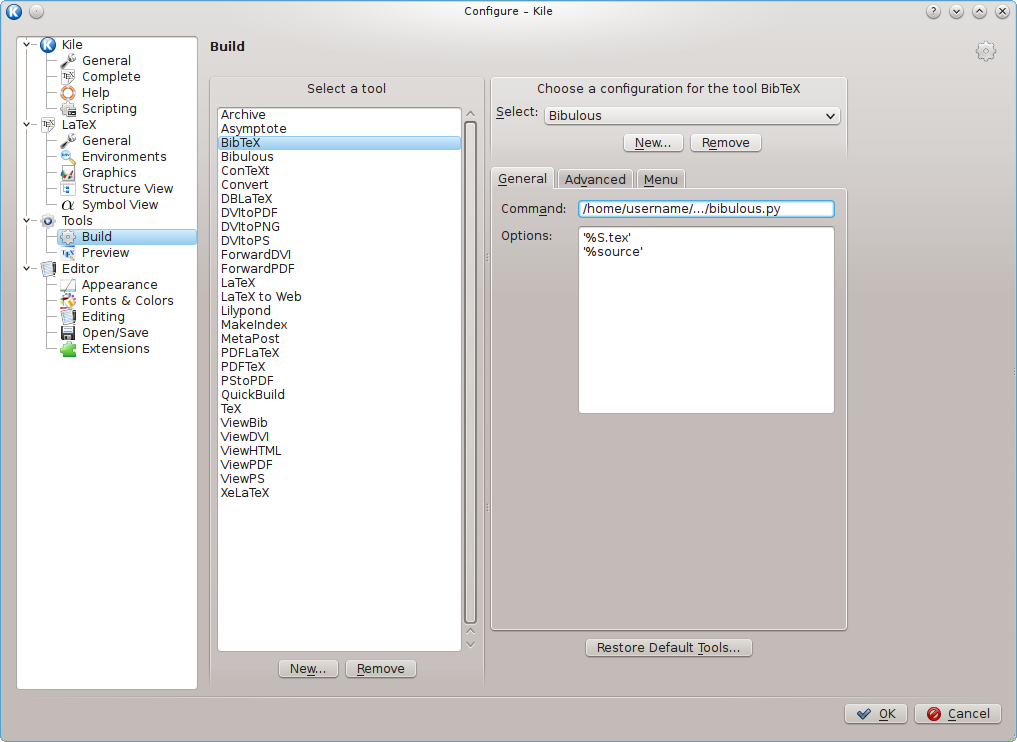
\includegraphics[width=0.490\linewidth]{screenshot_for_kile_instructions.png}

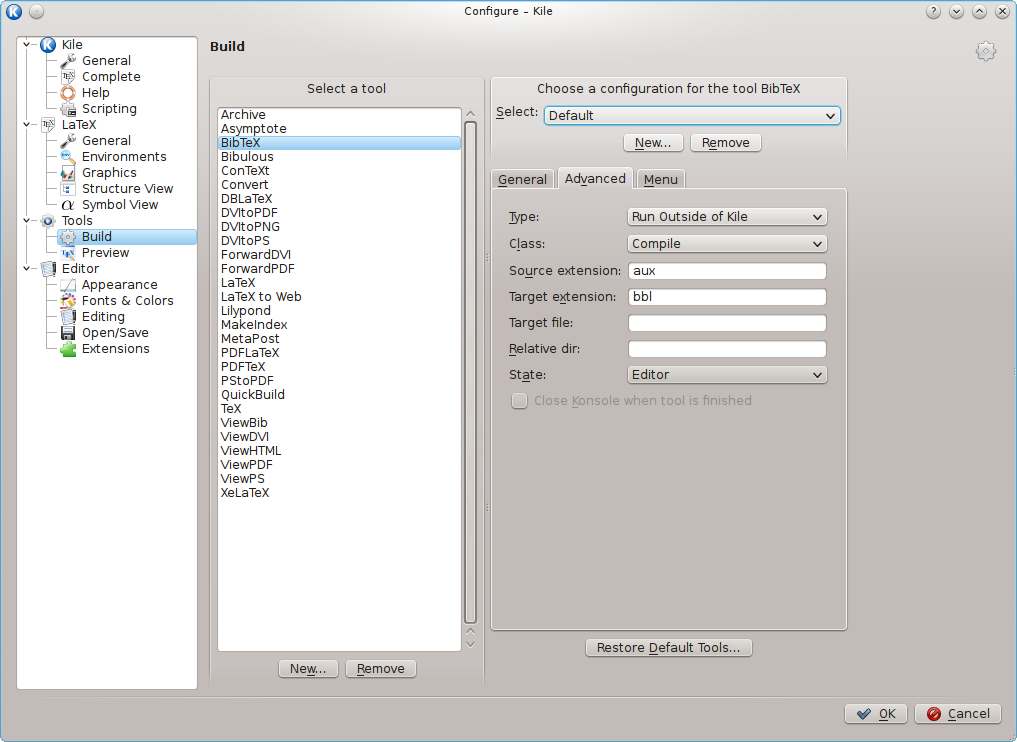
\includegraphics[width=0.490\linewidth]{screenshot_for_kile_instructions2.png}

That should be it. In case your default setup is different, you can also check the \code{Advanced} tab settings and verify that they are as shown in the second figure. (That is, \code{Source extension} is set to \code{aux}, and \code{Target extension} is set to \code{bbl}.)
\begin{enumerate}
\setcounter{enumi}{2}
\item {} 
Note that the following variables are accessible in Kile's \code{Options} field:

\begin{Verbatim}[commandchars=\\\{\}]
\%source = filename (i.e. filename with suffix but not path)
\%S = filename without suffix (and without path)
\%dir\_base = source file directory (source file's path without the filename)
\%dir\_target = target file directory (source file's path without the filename)
\end{Verbatim}

\end{enumerate}


\section{Modifying WinEdt5 to replace BibTeX with Bibulous}
\label{getting_started:modifying-winedt5-to-replace-bibtex-with-bibulous}\begin{enumerate}
\item {} 
Go to the menu \code{Options} \textgreater{} \code{Execution Modes}. In the \code{Console Applications} menu on the left hand side, select \code{BibTeX}. Then replace the three \code{Command Line} fields with the ones shown in the figure, replacing the files paths with the ones correct for your installation of Python and \code{bibulous.py}.

\end{enumerate}

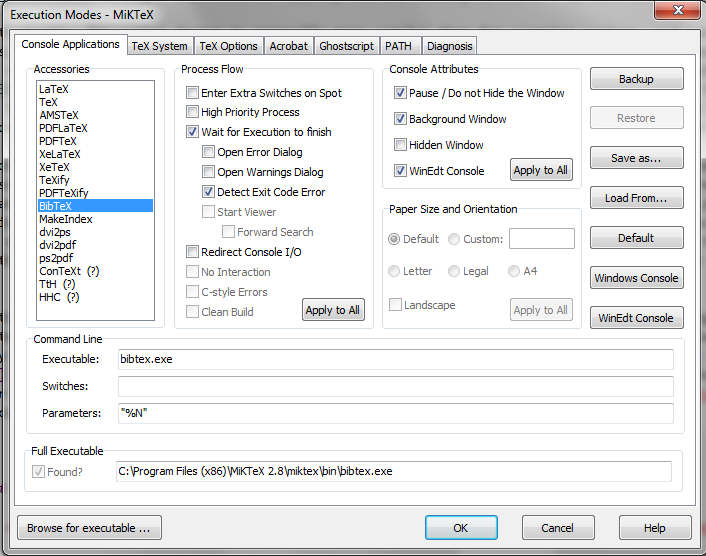
\includegraphics[width=0.490\linewidth]{original_Winedt5_setup.png}

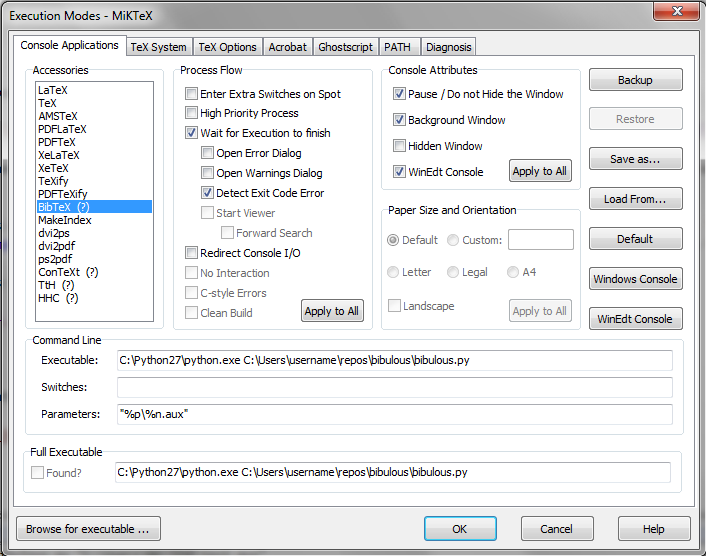
\includegraphics[width=0.490\linewidth]{modified_Winedt5_setup.png}
\begin{enumerate}
\setcounter{enumi}{1}
\item {} 
Note that the following are definitions of WinEdt registers:

\begin{Verbatim}[commandchars=\\\{\}]
\%f = full path of active file (= \%p/\%n.\%t)
\%n = name of the active file
\%p = the path of the active file
\%t = the extension of the active file
\%q = the path relative to the main file (i.e. for subdirectories)
\%b = WinEdt's local working directory (not the tex file directory)
\%B = path to the WinEdt executable file
\end{Verbatim}

\end{enumerate}


\chapter{Guidelines for writing bibliography style templates}
\label{guidelines_for_writing_style_templates:guidelines-for-writing-bibliography-style-templates}\label{guidelines_for_writing_style_templates::doc}

\section{Syntax}
\label{guidelines_for_writing_style_templates:syntax}\begin{enumerate}
\item {} 
Comments begin with \code{\#}, following the Python convention.

\item {} 
Each template file can have as many as five sections. None of the sections are required to be in the file, but any definitions in the file must be placed inside a section header so that the code knows how to deal with the definition. The four possible section headers are: TEMPLATES, SPECIAL-TEMPLATES, OPTIONS, VARIABLES, DEFINITIONS. And note that a section header is always placed by itself on a line and has a colon appended to it, as in \code{TEMPLATES:}.

\item {} 
The \code{TEMPLATES} section of the file contains template definitions for formatting references. The \code{SPECIAL-TEMPLATES} section contains definitions for creating variables within each database entry. The \code{OPTIONS} section contains definitions for various keywords that can be used to modify program behavior. The \code{VARIABLES} section contains user definitions for new variables to be made available. The difference between these definitions and those in \code{SPECIAL-TEMPLATES} is that the ones provided in the \code{VARIABLES} section are in-line Python code, whereas the former use templates. Finally, the \code{DEFINITIONS} section of the file contains Python-executable code that can then make functionality available in the form of template variables. (An example is provided in the \emph{Python API} section below.

\item {} 
All variable definitions within the TEMPLATES, SPECIAL-TEMPLATES, and OPTIONS sections use the variable name followed by whitespace, an equals sign, more whitespace, and then the definition itself. Thus the {[}whitespace+=+whitespace{]} expression is the delimiter between variable and definition, and is required syntax.

\item {} 
An ellipsis \code{...} at the end of a line indicates a line continuation. All whitespace following the ellipsis, and all whitespace preceding text on the next line, is removed from the resulting connected text.

\item {} 
An ellipsis in the middle of a line indicates an ``implicit loop''. For details, see the \emph{Examples for namelist formatting} section below.

\item {} 
Inside the \code{TEMPLATES} section, all of the variable definitions are intended to map to a database entrytype name. For example:

\begin{Verbatim}[commandchars=\\\{\}]
article = \textless{}au\textgreater{}, {}`{}`\textless{}title\textgreater{},'' \textless{}journal\textgreater{}, \textless{}volume\textgreater{}, \textless{}startpage\textgreater{}--\textless{}endpage\textgreater{} (\textless{}year\textgreater{}).
\end{Verbatim}

Here the \code{article} entrytype will be typeset so that the list of authors (\code{\textless{}au\textgreater{}}) is followed by the article title in double quotes, the journal name in standard font (i.e. not italics), the volume number, the page range, and the year.

\item {} 
A variable is indicated by angle brackets, as \code{\textless{}var\textgreater{}} and represents the contents of a field found within the bibliography database. Thus, when typesetting the bibliography, Bibulous will replace the variable \code{\textless{}authorlist\textgreater{}} with the string stored in the \code{authorlist} field of the current entry being formatted. An example list of typical variables one might use is:
\begin{quote}

\code{\textless{}au\textgreater{}}, \code{\textless{}booktitle\textgreater{}}, \code{\textless{}chapter\textgreater{}}, \code{\textless{}edition\textgreater{}}, \code{\textless{}ed\textgreater{}}, \code{\textless{}eid\textgreater{}}, \code{\textless{}endpage\textgreater{}}, \code{\textless{}institution\textgreater{}}, \code{\textless{}journal\textgreater{}}, \code{\textless{}nationality\textgreater{}}, \code{\textless{}note\textgreater{}}, \code{\textless{}number\textgreater{}}, \code{\textless{}organization\textgreater{}}, \code{\textless{}publisher\textgreater{}}, \code{\textless{}school\textgreater{}}, \code{\textless{}series\textgreater{}}, \code{\textless{}startpage\textgreater{}}, \code{\textless{}title\textgreater{}}, \code{\textless{}version\textgreater{}}, \code{\textless{}volume\textgreater{}}, \code{\textless{}year\textgreater{}}.
\end{quote}

This list is actually freely extensible. A user can add any additional variables needed, so that if a \code{video} field is used in a \code{.bib} database file, then this can be used within a formatted reference simply by placing \code{\textless{}video\textgreater{}} into the template wherever the information needs to be inserted.

\item {} 
Any variable placed within square brackets \code{{[}{]}} indicate that it is an optional variable --- it is not required that the database have that entry. While required entries that are not defined in the BibTeX database file (.bib file) are replaced with `???', and undefined optional variables are simply skipped. If a \code{\textbar{}} is present within the square brackets, it indicates an ``elseif'' clause. That is, if the template is \code{{[}\textless{}var1\textgreater{}\textbar{}\textless{}var2\textgreater{} and \textless{}var3\textgreater{}{]}}, then the code will look for \code{var1} as a field within the current database entry being formatted. If it does not find the entry, then it will try the next block, where it finds the two variables \code{var2} and \code{var3}. If both are defined, then the original template \code{{[}\textless{}var1\textgreater{}\textbar{}\textless{}var2\textgreater{} and \textless{}var3\textgreater{}{]}} is replaced with \code{\textless{}var2\textgreater{} and \textless{}var3\textgreater{}} (i.e. removing the square brackets) and proceeds to replace the two variables with their corresponding fields. If either one of \code{var2} or \code{var3} is undefined in the entry, then the entire optional {[}...{]} portion of the template is skipped.

\item {} 
If the \code{\textbar{}} symbol is used to create an empty last cell, as in \code{{[}\textless{}var1\textgreater{}\textbar{}\textless{}var2\textgreater{}\textbar{}{]}}, this indicates that while the individual cells within the optional block are themselves optional, it is required to have at least \_one\_ among the cells to be defined. Thus, \code{{[}\textless{}note\textgreater{}\textbar{}{]}} has the same meaning as simply \code{\textless{}note\textgreater{}} does.

\item {} 
Nesting of \code{{[}{]}} brackets is allowed, but the syntax becomes computationally expensive to parse, so that these structures should be used sparingly:

\item {} 
Users that need to use \code{{[}}, \code{{]}}, \code{\#}, \code{\textless{}}, \code{\textgreater{}}, or \code{\textbar{}} symbols as formatting elements within the reference list can implement them using some custom LaTeX-markup commands: \code{\{\textbackslash{}makeopenbracket\}}, \code{\{\textbackslash{}makehashsign\}}, \code{\{\textbackslash{}makeclosebracket\}}, \code{\{\textbackslash{}makegreaterthan\}}, \code{\{\textbackslash{}makelessthan\}}, or \code{\{\textbackslash{}makeverticalbar\}}. Note that the curly brackets used in each case are required.

\item {} 
In the \code{TEMPLATES} section of the file, if an entrytype format definition contains only another entrytype name on the right hand side of the \code{=}, i.e.:

\begin{Verbatim}[commandchars=\\\{\}]
\PYG{n}{inbook} \PYG{o}{=} \PYG{n}{incollection}
\end{Verbatim}

then this means that the existing \code{incollection} template should be copied for use with \code{inbook} entrytypes. (Note that \code{incollection} should be defined above this line in order for this to work.)

\item {} 
Note that several fields are defined by default which are \emph{not} directly from the bibliography database. These are \code{au}, \code{authorlist}, \code{citekey}, \code{citenum}, \code{ed}, \code{editorlist}, \code{endpage}, and \code{startpage}. These fields are derived from the original database file, but have been reformatted. See the \emph{Default Fields} section below.

\item {} 
Although the entrytype template definitions listed below are in alphabetical order, that can be put in any desired order within the file. (The exception to this rule is that if a definition consists of, for example:

\begin{Verbatim}[commandchars=\\\{\}]
\PYG{n}{inbook} \PYG{o}{=} \PYG{n}{incollection}
\end{Verbatim}

then the \code{incollection} template must already be defined. Also note that two entrytype names are special and so cannot be used on the left hand side of the equals sign here: \code{comment} and \code{preamble}.

\item {} 
A user wanting a localized form of quotation should use \code{\textbackslash{}enquote\{\textless{}title\textgreater{}\}} rather than \code{{}`{}`\textless{}title\textgreater{}''}, and add \code{\textbackslash{}usepackage\{csquotes\}} to the preamble of the LaTeX document.

\item {} 
In the \code{OPTIONS} section of the file are the formatting options. None of these definitions are required. The complete list is given in the \emph{Options keywords} section below, together with explanations of each.

\item {} 
The \code{SPECIAL-TEMPLATES} section is where users can define their own fields that get generated for every database entry evaluated. For example, the variable definition:

\begin{Verbatim}[commandchars=\\\{\}]
group = [\textless{}organization\textgreater{}\textbar{}\textless{}institution\textgreater{}\textbar{}\textless{}corporation\textgreater{}\textbar{}]

in the {}`{}`SPECIAL-TEMPLATES{}`{}` section will create a {}`{}`group{}`{}` field that can be used as the variable {}`{}`\textless{}group\textgreater{}{}`{}` within the regular {}`{}`TEMPLATES{}`{}` section of the file. This effectively allows users to create a shortcut. Where they could write out {}`{}`[\textless{}organization\textgreater{}\textbar{}\textless{}institution\textgreater{}\textbar{}\textless{}corporation\textgreater{}\textbar{}]{}`{}` inside each template that needs this structure, the special template definition allows them to replace each instance with a simple {}`{}`\textless{}group\textgreater{}{}`{}`.

Another example usage would be the following:::

author = [\textless{}著者名\textgreater{}\textbar{}\textless{}author-en\textgreater{}\textbar{}]

where the {}`{}`author{}`{}` field is actually redefined to include not only the *existing* author field, but also the fields {}`{}`著者名{}`{}` or {}`{}`author-en{}`{}`. That is, if the {}`{}`author{}`{}` field is missing in the database entry, the code next searches for the {}`{}`著者名{}`{}` field. If it finds it, then it will create an {}`{}`author{}`{}` field that contains a copy of the {}`{}`著者名{}`{}`'s field's contents. If the {}`{}`著者名{}`{}` is also missing, the code next searches for {}`{}`author-en{}`{}` and uses that fields contents to create the missing {}`{}`author{}`{}` field.
\end{Verbatim}

\item {} 
The order in which any definitions are placed within the special templates is important. For example, if a user has \code{au = \textless{}authorlist.format\_authorlist()\textgreater{}} and then below that defines \code{authorlist = \textless{}author.to\_namelist()\textgreater{}}, then the code will issue an error stating that \code{authorlist} is not defined when attempting to create the \code{au} variable. Since the definition for \code{au} assumes the presence of the \code{authorlist} variable, the latter definition must be placed above it.

\end{enumerate}


\section{Default Fields}
\label{guidelines_for_writing_style_templates:default-fields}
A complete of the existing default fields is::

\begin{Verbatim}[commandchars=\\\{\}]
\PYG{n}{au}
\PYG{n}{authorlist}
\PYG{n}{citekey}
\PYG{n}{citenum}
\PYG{n}{ed}
\PYG{n}{editorlist}
\end{Verbatim}

Each of these default fields are defined as ``special templates''. If a user defines a special template with the same name as one of the above, then the default is overwritten with the user's version. The definitions of these six default special templates are::

\begin{Verbatim}[commandchars=\\\{\}]
authorlist = \textless{}author.to\_namelist()\textgreater{}
editorlist = \textless{}editor.to\_namelist()\textgreater{}
citelabel = \textless{}citenum.remove\_leading\_zeros()\textgreater{}
sortkey = \textless{}citenum\textgreater{}
au = \textless{}authorlist.format\_authorlist()\textgreater{}
ed = \textless{}editorlist.format\_editorlist()\textgreater{}
\end{Verbatim}

Note that the ordering of definitions is important. The following summarizes what these definitions are used for.

\textbf{authorlist} creates a list of dictionaries (one dictionary for each author name found within the database entry's \code{author} field). Each name dictionary has keys ``first'', ``middle'', ``prefix'', ``last'', and ``suffix'', where each of these keys is optional except for ``last''. Thus, a user can access the first and last name of the first author in the database entry using \code{\textless{}authorlist.0.first\textgreater{} \textless{}authorlist.0.last\textgreater{}}. To access the middle name(s) of the second author, use \code{\textless{}authorlist.1.middle\textgreater{}}.

\textbf{editorlist} behaves exactly as \code{authorlist} but derives its list of names from the database entry's \code{editor} field rather than \code{author} field.

\textbf{citelabel} is the thing that appears at the front of the formatted reference, and is identical to the citation label used in the manuscript to point to the item in the reference list. In technical journal articles, this is typically just a number, as in the default definition \code{\textless{}citenum.remove\_leading\_zeros()\textgreater{}}. The number used here for the label indicates the order in which the entry was cited. Since the variable \code{citenum} is a string that contains leading zeros, so that the entries are properly sorted in order of 001, 002, ..., 009, 010, 011, ... and not in the strict alphabetical order of 1, 10, 11, ..., 19, 2, 20, 21, .... But for a citation label, the leading zeros are unsightly, and so we use the \code{.remove\_leading\_zeros()} operator to remove them from the string before creating the label.

\textbf{sortkey} is the string used to sort the entry within the reference list. For technical journal articles, what is generally wanted is just the citation order, as indicated by the \code{\textless{}citenum\textgreater{}} variable.

\textbf{au} is the string representing the formatted list of author names. In the default definition shown above, the name list is a standard form, and so simply uses the \code{.format\_authorlist()} operator. Generally, this operator creates name lists that have the form ``firstauthor'' for only one author, ``firstauthor and secondauthor'' if only two authors, ``firstauthor, secondauthor, ..., and lastauthor'' if more than two authors but less than the maximum, and ``firstauthor, secondauthor, ..., minauthor, et al.'' if more than the maximum allowed number of authors. Which author in the list is ``minauthor'' is defined using the \code{minauthors} option keyword. The maximum number of allowed authors is set by the \code{maxauthors} option keyword.

\textbf{ed} follows the same basic structure as \code{au}, but uses the \code{maxeditors} and \code{mineditors} keywords.


\subsection{Operators}
\label{guidelines_for_writing_style_templates:operators}
One can use the ``dot'' operator inside a variable name, as in \code{\textless{}authorname.0.last.initial()\textgreater{}'' to perform any one of four functions: a explicit numerical index (the {}`{}`0} shown here), an implicit numerical index (using \code{.n} or \code{.N}, for which see section \emph{Examples for namelist formatting} below for details), a dictionary lookup (the \code{last} used here), or the application of an operator (in this case, the \code{.initial()} operator which is used to reduce a name to its initial). A numerical index must apply to a list-type of variable, and a key index must apply to a dict-type of variable (i.e. a dictionary).

The complete list of operators available is::

\begin{Verbatim}[commandchars=\\\{\}]
.compress()
.format\_authorlist()
.format\_editorlist()
.frenchinitial()
.if\_singular(var1,var2,var3)
.initial()
.monthabbrev()
.monthname()
.ordinal()
.remove\_leading\_zeros()
.sentence\_case()
.tie()
.to\_namelist()
\end{Verbatim}

The function of each operator is summarized below.

\textbf{.compress()} removes any whitespace found within the string. This is useful for generating namelists where the format requires ``tight'' spacing. An example would be ``RMA Azzam'', where the three initials are grouped together without spacing. And example template for generating this type of name would be:

\begin{Verbatim}[commandchars=\\\{\}]
\textless{}authorlist.0.first\textgreater{}\textless{}authorlist.0.middle.initial().compress()\textgreater{} \textless{}authorlist.0.last\textgreater{}
\end{Verbatim}

Without the \code{.compress()} operator, the name would come out as ``RM A Azzam'', where the two middle name initials ``M'' amnd ``A'' are spaced apart from one another by default.

\textbf{.format\_authorlist()} operates on a list of dictionaries type of variable (a namelist), and uses the keyword-based default formatting scheme to create a formatted string of names. The complete list keywords that it work with is: \code{etal\_message}, \code{maxauthors}, \code{minauthors}, \code{namelist\_format}, \code{period\_after\_initial}, \code{terse\_inits}, \code{use\_firstname\_initials}, \code{use\_name\_ties}. The default formatter, while fast, is not very flexible, so that users looking for more customizability will want to make use of Bibulous' implicit-index and implicit-loop based definitions. See the \emph{Example definitions for namelist formatting} section below.

\textbf{.format\_editorlist()} operates on a list of dictionaries type of variable (a namelist), and uses the keyword-based default formatting scheme to create a formatted string of names.  The complete list keywords that it work with is: \code{etal\_message}, \code{maxeditors}, \code{mineditors}, \code{namelist\_format}, \code{period\_after\_initial}, \code{terse\_inits}, \code{use\_firstname\_initials}, \code{use\_name\_ties}. (The difference with the \code{.format\_authorlist()} operator is that it uses \code{maxeditors} and \code{mineditors} rather than \code{maxauthors} and \code{minauthors}) The default formatter, while fast, is not very flexible, so that users looking for more customizability will want to make use of Bibulous' implicit-index and implicit-loop based definitions. See the \emph{Example definitions for namelist formatting} section below.

\textbf{.frenchinitial()} is an alternative form of the \code{.initial()} operator that has slightly different behavior. If a name begins with one of the digraphs
``Ch'', ``Gn'', ``Ll'', ``Ph'', ``Ss'', or ``Th'', then the initial will truncate the name after the digraph instead of after the first letter.

\textbf{.if\_singular(var1,var2,var3)} is an operator which inserts \code{var2} if \code{var1} has only one element, but \code{var3} if \code{var1} has more than one element. Here \code{var1} is assumed to be a list-type of variable, and \code{var2} and \code{var3} are assumed to be either fields present within the database entry or variables defined in the \code{SPECIAL-TEMPLATES} section of the file.

\textbf{.initial()} will truncate the string to its first letter. Note that if a name begins with a LaTeX markup character, such as \code{\{\textbackslash{}'E\}}, then the operator will convert the input string to its best attempt at a Unicode-equivalent (without character markup) prior to performing the truncation. Thus, applying the \code{.initial()} operator to the name \code{\{\textbackslash{}v\{Z\}\}ukauskas} will produce the initialized form ``Ž''.

\textbf{.monthabbrev()} assumes that the input field is a number from 1 to 12, and converts the numerical input into the abbreviated month according to the user's current locale. If the system cannot determine the user's locale, the operator will default to using the American English locale, which replaces the numerical field operated on with one of ``Jan'', ``Feb'', ``Mar'', ``Apr'', ``May'', ``Jun'', ``Jul'', ``Aug'', ``Sep'', ``Oct'', ``Nov'', or ``Dec'' according to the field's value. Thus, if the bibliography database entry has a field \code{month = 11}, and the template has the form \code{\textless{}month.monthabbrev()\textgreater{}}, then the template will be replaced with ``Nov'' for the default locale. For users with locale ``Japan'', this same operator will return ``11月''.

\textbf{.monthname()} behaves much like \code{.monthabbrev()} but rather than using an abbreviated form for the month's name, it uses the full form. Thus if the bibliography database entry has a field \code{month = 3}, and the template has the form \code{\textless{}month.monthname()\textgreater{}}, then the template variable will be replaced with ``March'' for the default locale. For users with locale ``Norway'', this same operator will return ``Mars''.

\textbf{.ordinal()} creates an ``ordinal'' from a numerical field. Thus, if the field operated on is ``1'', ``2'', ``3'', or ``4'', then the operator will replace the template with ``1st'', ``2nd'', ``3rd'' or ``4th''. Any number above 4 simply has ``th'' appended to the end of it. Currently Bibulous does not support non-English locales for this function. (Anyone having suggestions of how this may be implemented without too much fuss should contact us!)

\textbf{.remove\_leading\_zeros()} deletes any zeros from the front of the field operated on. Thus ``003'' will be returned as ``3''.

\textbf{.sentence\_case()} reduces the lower case any characters in the field, except for the initial letter and any letters protected within a pair of curly braces. For example, if the database entry has \code{title = \{Understanding Bohmian mechanics\}} and the template has the form \code{\textless{}title.sentence\_case()\textgreater{}}, then the template variable will be replaced with ``Understanding bohmian mechanics''. However, if the entry has \code{title = \{Understanding \{B\}ohmian mechanics\}}, the result will be ``Understanding \{B\}ohmian mechanics''.

\textbf{.tie()} replaces any spaces with an unbreakable space. Thus, ``R. M. A.'' becomes ``R.\textasciitilde{}M.\textasciitilde{}A.''. An example use of this operator would be the following template::

\begin{Verbatim}[commandchars=\\\{\}]
authorname = [\textless{}authorlist.n.first.initial()\textgreater{}.\textasciitilde{}][\textless{}authorlist.n.middle.initial().tie()\textgreater{}. ]...
             [\textless{}authorlist.n.prefix\textgreater{}\textasciitilde{}]\textless{}authorlist.n.last\textgreater{}[, \textless{}authorlist.n.suffix\textgreater{}]
\end{Verbatim}

\textbf{.to\_namelist()} parses the field (assumed to be a BibTeX-format ``and''-delimited list of names) into a Bibulous-format namelist (i.e. a list of dictionaries).


\section{Options keywords}
\label{guidelines_for_writing_style_templates:options-keywords}
A complete list of existing options keywords, together with their default definitions, is::

\begin{Verbatim}[commandchars=\\\{\}]
allow\_scripts = False
backrefs = False
backrefstyle = none
bibitemsep = None
case\_sensitive\_field\_names = False
edmsg1 = , ed.
edmsg2 = , eds
etal\_message = , \PYGZbs{}\PYGZbs{}textit\PYGZob{}et al.\PYGZcb{}
maxauthors = 9
maxeditors = 5
minauthors = 9
mineditors = 5
namelist\_format = first\_name\_first
period\_after\_initial = True
procspie\_as\_journal = False
show\_urls = False
sort\_case = True
terse\_inits = False
undefstr = ???
use\_abbrevs = True
use\_citeextract = True
use\_firstname\_initials = True
use\_name\_ties = False
\end{Verbatim}

Each of the keywords is summarized below.

\textbf{allow\_scripts} {[}default value: False{]} tells Bibulous whether to allow the evaluation of Python code in the VARIABLES and DEFINITIONS sections of \code{.bst} files. It is important for users to realize that evaluating external code in this way is a security risk, and so they should not set \code{allow\_scripts = True} when inserting code that they do not trust. However, as an additional security precaution, Bibulous prevents most security-sensitive operations from being used within its Python API.

\textbf{backrefs} {[}default value: False{]} THIS KEYWORD IS NOT YET IMPLEMENTED

\textbf{backrefstyle} {[}default value: none{]} THIS KEYWORD IS NOT YET IMPLEMENTED

\textbf{bibitemsep} {[}default value: None{]} provides users a means to change the amount of vertical separation that LaTeX sets between entries in the reference list. For example, users wanting a more compact list can define \code{bibitemsep = 0pt}.

\textbf{case\_sensitive\_field\_names} {[}default value: False{]} tells Bibulous whether to consider, for example, a field named ``Author'' as being distinct from ``author''.

\textbf{edmsg1} {[}default value: , ed.{]} provides a string to use after a list of editor names, for the case when only one editor is present.

\textbf{edmsg2} {[}default value: , eds{]} provides a string to use after a list of editor names, for the case when multiple editors are present.

\textbf{etal\_message} {[}default value: , \textbackslash{}textit\{et al.\}{]} provides a string to use after a truncated namelist (for example, when the number of authors exceeds the value given by the \code{maxauthors} keyword).

\textbf{maxauthors} {[}default value: 9{]} provides the maximum number of allowed names in the formatted list of authors. If the number of names is more than this, then the list of names is truncated to \code{minauthors} and the \code{etal\_message} is appended to the result. (This keyword is only used within the \code{.format\_namelist()} operator.)

\textbf{maxeditors} {[}default value: 5{]} provides the maximum number of allowed names in the formatted list of editors. If the number of names is more than this, then the list of names is truncated to \code{mineditors} and the \code{etal\_message} is appended to the result. (This keyword is only used within the \code{.format\_namelist()} operator.)

\textbf{minauthors} {[}default value: 9{]} provides the minimum number of author names to use when truncating an overlength author name list. (This keyword is only used within the \code{.format\_namelist()} operator.)

\textbf{mineditors} {[}default value: 5{]} provides the minimum number of editor names to use when truncating an overlength author name list. (This keyword is only used within the \code{.format\_namelist()} operator.)

\textbf{namelist\_format} {[}default value: first\_name\_first, allowed values: \{first\_name\_first, last\_name\_first\}{]} defines how the formatted list of names should appear. If \code{namelist\_format = first\_name\_first} then the individual names will appear in the order ``firstname middle prefix last, suffix''. If \code{namelist\_format = last\_name\_first} then the individual names will appear in the order ``prefix last, firstname middle, suffix''. (This keyword is only used within the \code{.format\_namelist()} operator.)

\textbf{period\_after\_initial} {[}default value: True{]} tells the \code{.format\_namelist()} operator whether to place a period after each initial of an individual's name. Thus, if \code{period\_after\_initial = True}, a name will appear as ``R. M. A. Azzam'', but if \code{False} will appear as ``R M A Azzam''. (This keyword is only used within the \code{.format\_namelist()} operator.)

\textbf{procspie\_as\_journal} {[}default value: False{]} The ``Proceedings of SPIE'' are treated as special by the journals of the Optical Society of America. That is, they format these proceedings (and only these) in the same way that they do journal articles. Thus, a special keyword is required to allow this behavior.

\textbf{show\_urls} {[}default value: False{]} informs Bibulous whether or not to use the \code{hyperref} package for placing hyperlinks into the formatted reference.

\textbf{sort\_case} {[}default value: True{]} informs Bibulous whether or not to use case-sensitive sorting of reference keys.

\textbf{terse\_inits} {[}default value: False{]} tells the \code{.format\_namelist()} operator whether to compress together the initials of an individual's name. Thus, if \code{terse\_inits = True}, a name will appear as ``RMA Azzam'', but if \code{False} will appear as ``R. M. A. Azzam''. (This keyword is only used within the \code{.format\_namelist()} operator.)

\textbf{undefstr} {[}default value: ???{]} informs Bibulous what kind of warning message to print when a required field is missing in the database entry.

\textbf{use\_abbrevs} {[}default value: True{]} tells Bibulous whether or not to use the abbreviations defined in the bibliography database. (Used for debugging.)

\textbf{use\_citeextract} {[}default value: True{]} tells Bibulous whether to perform ``citation extraction'', which creates a small database of only the cited items from among the complete database provided in the \code{.aux} file.

\textbf{use\_firstname\_initials} {[}default value: True{]} Whether or not to initialize the first names of authors in the formatted authors list. (This keyword is only used within the \code{.format\_namelist()} operator.)

\textbf{use\_name\_ties} {[}default value: False{]} Whether or not to replace spaces with unbreakable spaces (i.e. ``R. M. A. Azzam'' or ``R.\textasciitilde{}M.\textasciitilde{}A. Azzam'') inside names in the name list. (This keyword is only used within the \code{.format\_namelist()} operator.)


\section{Examples for namelist formatting}
\label{guidelines_for_writing_style_templates:examples-for-namelist-formatting}
The following code provides an example usage of implicit indexing within an implicit loop structure::

\begin{Verbatim}[commandchars=\\\{\}]
authorlist = \textless{}author.to\_namelist()\textgreater{}
editorlist = \textless{}editor.to\_namelist()\textgreater{}
authorname.n = [\textless{}authorlist.n.first.initial()\textgreater{}. ][\textless{}authorlist.n.middle.initial()\textgreater{}. ]...
               [\textless{}authorlist.n.prefix\textgreater{} ]\textless{}authorlist.n.last\textgreater{}[, \textless{}authorlist.n.suffix\textgreater{}]
au = \textless{}authorname.0\textgreater{}, ...,\PYGZob{} and \PYGZcb{}\textless{}authorname.9\textgreater{}
editorname.n = [\textless{}editorlist.n.first.initial()\textgreater{}. ][\textless{}editorlist.n.middle.initial()\textgreater{}. ]...
               [\textless{}editorlist.n.prefix\textgreater{} ]\textless{}editorlist.n.last\textgreater{}[, \textless{}editorlist.n.suffix\textgreater{}]
ed = \textless{}editorname.0\textgreater{}, ...,\PYGZob{} and \PYGZcb{}\textless{}editorname.2\textgreater{}
\end{Verbatim}

Here the \code{authorlist} and \code{editorlist} definitions create namelist variables from the \code{author} and \code{editor} fields in the entry (if they exist). Next, the implicitly-indexed \code{authorname.n} cannot operate except within an implicit loop, and so we should describe that first. It is easier to describe the functionality of the \code{ed} template than the \code{au} one, as it has a smaller number of allowed names. The \code{ed} template has the definition:

\begin{Verbatim}[commandchars=\\\{\}]
\textless{}editorname.0\textgreater{}, ...,\PYGZob{} and \PYGZcb{}\textless{}editorname.2\textgreater{}
\end{Verbatim}

which simplifies to \code{\textless{}editorname.0\textgreater{}} when there is only one editor in the database entry, and:

\begin{Verbatim}[commandchars=\\\{\}]
\textless{}editorname.0\textgreater{} and \textless{}editorname.1\textgreater{}
\end{Verbatim}

when there are only two. Here the separator {}`{}` and {}`{}` comes from the \code{\{ and \}} placed at the right hand side of the implicit loop. For three editors, the implicit loop expands the template to:

\begin{Verbatim}[commandchars=\\\{\}]
\textless{}editorname.0\textgreater{}, \textless{}editorname.1\textgreater{}, and \textless{}editorname.2\textgreater{}
\end{Verbatim}

where this time the comma alone is used as the first delimiter, as it is outside the enclosed braces. For the final element, both the comma and the \code{\{ and \}} at the right hand side of the implicit loop are used as the final delimiter. Since the template does not specify the format for more than three editor names, the code builds an \emph{et al.} construction when there more than this number of names, so that the result becomes:

\begin{Verbatim}[commandchars=\\\{\}]
\textless{}editorname.0\textgreater{}, \textless{}editorname.1\textgreater{}, \textless{}editorname.2\textgreater{}, \PYGZbs{}textit\PYGZob{}et al.\PYGZcb{}
\end{Verbatim}

where the form of the string \code{\textbackslash{}textit\{, et. al\}} is specified by the \code{etal\_message} keyword option.

Thus, the implicit loop has filled out a unique template based on the number of editors it finds within the database entry. The next step is to use the implicitly-indexed \code{editorname} to complete building out the template. The latter template is defined as:

\begin{Verbatim}[commandchars=\\\{\}]
editorname.n = [\textless{}editorlist.n.first.initial()\textgreater{}. ][\textless{}editorlist.n.middle.initial()\textgreater{}. ]...
               [\textless{}editorlist.n.prefix\textgreater{} ]\textless{}editorlist.n.last\textgreater{}[, \textless{}editorlist.n.suffix\textgreater{}]
\end{Verbatim}

so that a template variable of the form {\color{red}\bfseries{}{}`{}`}\textless{}editorname.0\textgreater{}'' is replaced with:

\begin{Verbatim}[commandchars=\\\{\}]
[\textless{}editorlist.0.first.initial()\textgreater{}. ][\textless{}editorlist.0.middle.initial()\textgreater{}. ]...
[\textless{}editorlist.0.prefix\textgreater{} ]\textless{}editorlist.0.last\textgreater{}[, \textless{}editorlist.0.suffix\textgreater{}]
\end{Verbatim}

That is, the implicit index \code{.n} is everywhere replaced with the explicit index \code{0}. For the case of a database entry containing two editor names, the final template will thus have the form:

\begin{Verbatim}[commandchars=\\\{\}]
[\textless{}editorlist.0.first.initial()\textgreater{}. ][\textless{}editorlist.0.middle.initial()\textgreater{}. ]...
[\textless{}editorlist.0.prefix\textgreater{} ]\textless{}editorlist.0.last\textgreater{}[, \textless{}editorlist.0.suffix\textgreater{}] and ...
[\textless{}editorlist.1.first.initial()\textgreater{}. ][\textless{}editorlist.1.middle.initial()\textgreater{}. ]...
[\textless{}editorlist.1.prefix\textgreater{} ]\textless{}editorlist.1.last\textgreater{}[, \textless{}editorlist.1.suffix\textgreater{}]
\end{Verbatim}

With this template now complete, the code begins to evaluate the entry and replace the individual variables with their corresponding database fields.


\section{Python API}
\label{guidelines_for_writing_style_templates:python-api}
Bibulous also provides to users an extensible Python interface allowing users to directly manipulate Bibulous' internal data structures. These use the \code{VARIABLES} and \code{DEFINITIONS} sections of the file, as shown below. For the \code{{}`VARIABLES} section, a variable name is defined (the first example below defines the variable \code{year\_bce}, while the second example below defines \code{pagerange}). On the right hand side of the definition, however, is a Python function call. This is different from the other sections of the BST file, which use template syntax. Any variable defined in this way within the \code{VARIABLES} section can then be accessed as a template variable (i.e. \code{\textless{}year\_bce\textgreater{}}) within the \code{TEMPLATES} section of the file. Two example uses are shown below.

To allow Bibulous to read the \code{VARIABLES} and \code{DEFINITIONS} sections of the file, users must set the option keyword \code{allow\_scripts} to True.

\textbf{First example: a custom yearstyle}. For a bibliography containing works from authors dating from before year 0, a common approach is to append ``BC'' to the year number, and for positive-numbered years, appending ``AD''. More recently, the convention has been to append ``BCE'' and ``CE'' rather than ``BC'' and ``AD''. The example defines an option keyword \code{yearstyle} that allows users to switch between one style (BC/AD) and the other (BCE/CE). This keyword is accessed by placing \code{options} as an argument to the \code{format\_yearstyle()} function defining the variable \code{year\_bce}. Inside the function, it can then check the options dictionary for the \code{yearstyle} keyword and determine which convention to use.

The \code{format\_yearstyle()} function itself is straightforward. It first checks whether the entry has a \code{year} field. If not, then it returns \code{None}, indicating that the function's result is undefined. If it finds a \code{year} field, then it checks to see whether it corresponds to an integer. If not, then it returns the field as-is. (Perhaps a user defines his \code{year} fields as \code{45 BCE} with the BCE already written out inside the field?) If it finds an integer value, then it determines which style to use (BC/AD or BCE/CE). If the year number is negative then it appends ``BC'' or ``BCE to the end. If the year number is positive then it appends ``AD'' or ``CE to the end, depending on the convention chosen.

Example:

\begin{Verbatim}[commandchars=\\\{\}]
OPTIONS:
allow\_scripts = True
yearstyle = BCE/CE

VARIABLES:
year\_bce = format\_yearstyle(entry, options)

DEFINITIONS:
\#\# NOTE! Only Unix-style line endings are allowed here.
def format\_yearstyle(entry, options):
    '''
    Append "BC or "AD" to "year", depending on whether the year is positive or negative.
    If the option "yearstyle" is set to "BCE/CE", then use "BCE" and "CE" instead of "BC"
    and "AD".
    '''

    if ('year' not in entry):
        return(options['undefstr'])

    \#\# First check that the year string is an integer. If not an integer, then just return
    \#\# the field itself.
    if not str\_is\_integer(entry['year']):
        return(entry['year'])

    yearnum = int(entry['year'])

    if (yearnum \textless{} 0):
        if (options['yearstyle'] == 'BCE/CE'):
            suffix = 'BCE'
        else:
            suffix = 'BC'
        \#\# The "[1:]" here removes the minus sign.
        result = str(yearnum)[1:] + ' ' + suffix
    elif (yearnum == 0):
        result = str(yearnum)
    else:
        if (options['yearstyle'] == 'BCE/CE'):
            suffix = 'CE'
        else:
            suffix = 'AD'
        result = str(yearnum) + ' ' + suffix

    return(result)
\end{Verbatim}

\textbf{Second example: a custom pagestyle}. For a bibliography containing works from magazines, it is not uncommon to find articles with large gaps in page numbers. Here is an example bibliography database entry:

\begin{Verbatim}[commandchars=\\\{\}]
@article\PYGZob{}stewart,
title = \PYGZob{}Interview with Walter Stewart\PYGZcb{},
author = \PYGZob{}Doug Stewart\PYGZcb{},
journal = \PYGZob{}Omni\PYGZcb{},
year = \PYGZob{}1989\PYGZcb{},
volume = \PYGZob{}11\PYGZcb{},
number = \PYGZob{}5\PYGZcb{},
pages = \PYGZob{}64--66, 87--92, 94\PYGZcb{}
\PYGZcb{}
\end{Verbatim}

where we can see that the article was broken into three sections in order to fit the editors' formatting requirements. Many bibliography styles require a starting and ending page, but these are misleading when the article is broken across pages in this way. Thus, a user may want to have the option that if a comma is found within the \code{pages} field of an entry then it should be displayed as-is. If no comma is found, then it simply returns the standard startpage--endpage pair.

To make this work, first the option \code{allow\_scripts} must be set to true. Next, a new \code{pagerange} variable is defined, so that it can be accessed in the \code{TEMPLATES} section of the file as \code{\textless{}pagerange\textgreater{}}. The variable is defined as the return value of the function \code{format\_pagerange()} given in the \code{DEFINITIONS} section. The defined function first checks to see if there is a \code{pages} field defined in the entry. If not, then it returns None, so that the \code{pagerange} variable will also be undefined. If it finds the \code{pages} field, it looks to see if there is a comma present. If so, it returns the field as-is. If not, it looks for the \code{endpage} variable (generated by default by Bibulous from the \code{pages} field). If present, then the function returns a startpage--endpage pair. If \code{endpage} is not present, then it returns only the \code{startpage} variable.

Example:

\begin{Verbatim}[commandchars=\\\{\}]
OPTIONS:
allow\_scripts = True

VARIABLES:
pagerange = format\_pagerange(entry, options)

DEFINITIONS:
def format\_pagerange(entry, options):
    '''
    If the "pages" field is comma-delimited, then return the pages field as-is. Otherwise
    return the standard startpage--endpage range.
    '''

    if not ('pages' in entry):
        return(None)
    elif (',' in entry['pages']):
        return(entry['pages'])
    elif ('endpage' in entry):
        return(entry['startpage']--entry['endpage'])
    else:
        return(entry['startpage'])
\end{Verbatim}


\chapter{Instructions on how to report a bug to the Bibulous development team}
\label{instructions_for_reporting_bugs:instructions-on-how-to-report-a-bug-to-the-bibulous-development-team}\label{instructions_for_reporting_bugs::doc}

\section{Where to report a bug}
\label{instructions_for_reporting_bugs:where-to-report-a-bug}
Send an email to the \code{users\_mailing\_list}. Once it's confirmed as a bug, someone, possibly you, can enter it into the issue tracker. (Or if you're pretty sure about the bug, go ahead and post directly to the developers mailing list, \code{developers\_mailing\_list}. But if you're not sure, it's better to post to {[}\code{users mailing list}{]} first; someone there can tell you whether the behavior you encountered is expected or not.)


\section{How to report a bug}
\label{instructions_for_reporting_bugs:how-to-report-a-bug}
First, make sure it's a bug. If Bibulous does not behave the way you expect, look in the documentation and mailing list archives for evidence that it should behave the way you expect. If the documentation and archives do not contain enough information to tell you whether the behavior is a bug or is expected behavior, go ahead and ask on the users mailing list first \code{users\_mailing\_list}. Also check that you are running the most recent version of Bibulous. It may be that the bug has already been fixed.

Once you've established that it's a bug, the most important thing you can do is come up with a simple description and reproduction recipe. For example, if the bug, as you initially found it, involves five files over ten commits, try to make it happen with just one file and one commit. The simpler the reproduction recipe, the more likely a developer is to successfully reproduce the bug and fix it.

When you write up the reproduction recipe, don't just write a prose description of what you did to make the bug happen. Instead, give a copy of the exact series of commands you ran, and their output. Use cut-and-paste to do this. If there are files involved, be sure to include the names of the files, and even their content if you think it might be relevant. The very best thing is to package your reproduction recipe as a script, that helps a lot.

In addition to the reproduction recipe, we'll also need a complete description of the environment in which you reproduced the bug. That means:
\begin{itemize}
\item {} 
Your operating system

\item {} 
The Python version you are running under.

\item {} 
The release and/or revision of Bibulous.

\item {} 
Anything else that could possibly be relevant. Err on the side of too much information, rather than too little.

\end{itemize}

Once you have all this, you're ready to write the report. Start out with a clear description of what the bug is. That is, say how you expected Bibulous to behave, and contrast that with how it actually behaved. While the bug may seem obvious to you, it may not be so obvious to someone else, so it's best to avoid a guessing game. Follow that with the environment description, and the reproduction recipe. If you also want to include speculation as to the cause, and even suggest how the code may be modified to fix the bug, that's great.

Post all of this information to the developers mailing list, \code{developers\_mailing\_list}, or if you have already been there and been asked to file an issue, then go to the Issue Tracker and follow the instructions there.

Thanks! It's a lot of work to file an effective bug report, but a good report can save hours of a developer's time, and make the bug much more likely to get fixed.


\chapter{Developer guide}
\label{developer_guide::doc}\label{developer_guide:developer-guide}

\section{Guidelines and notes for Python coding style}
\label{developer_guide:guidelines-and-notes-for-python-coding-style}\begin{enumerate}
\item {} 
Note that one can mix 8-bit Python strings (ASCII text) with UTF-8 encoded text as long as the 8-bit string contains only ASCII characters.

\item {} 
Keep in mind when running into Unicode errors: reading a line of text from a file produces a line of bytes and not characters. To decode the bytes into a string of characters, you need to know the encoding.

\item {} 
There are a couple of minor points where the Bibulous coding standards deviates from Python's PEP8:
\begin{enumerate}
\item {} 
A line width of 120 is the standard (not 80).

\item {} 
In general, statements that evaluate to a boolean are placed within parentheses (i.e. \code{if (a \textless{} b):} rather than \code{if a \textless{} b:}).

\end{enumerate}

\item {} 
Many developers prefer to spread out code among a large number of small files, but Bibulous is currently organized in a single large file. This is partly because there is no large block of code that fits by itself so that a separate file makes sense. (Parsing of \code{.bib} files, for example, only requires a couple hundred lines.

\end{enumerate}


\section{Overall project strategy and code structure}
\label{developer_guide:overall-project-strategy-and-code-structure}
The basic function of BibTeX is to accept an \code{.aux} file as input and to produce a \code{.bbl} file as output. The \code{aux} file contains all of the citation information as well as the filenames for the bibliography database file (\code{.bib}) and the style file (\code{.bst}).

The basic program flow is as follows:
\begin{enumerate}
\item {} 
Read the \code{.aux} file and get the names of the bibliography databases (\code{.bib} files), the style templates (\code{.bst} files) to use, together with the entire set of citations.

\item {} 
Read in the Bibulous style template file as a dictionary (\code{bstdict}).

\item {} 
If the \code{use\_citeextract} keyword is set to True, and if an ``extracted'' database file exists, then compare the citations in the extracted database against those in the \code{.aux} file. If there are any differences, then re-extract the database. Otherwise, use the extracted database rather than the full one specified in the \code{.aux} file.

\item {} 
Read in all of the bibliography database files into one long dictionary (\code{bibdata}), replacing any abbreviations with their full form. In an ``extracted'' database, all entries are parsed, whereas in any other type of database file, only those entries whose keywords are found in the citation list are actually parsed. All other entries have their data saved as unparsed strings. Cross-referenced data is \emph{not} yet inserted at this point. That is delayed until the time of writing the BBL file in order to speed up parsing. It is only then that the cross-referenced entries have their data parsed into dictionary form.

\item {} 
Now that all the information is collected, we can generate the \code{.bbl} file. Create the list of sortkeys, then go through each corresponding citation key in turn, and find the corresponding entry key in \code{bibdata}. If there is crossref data, then fill in missing values here. Also create the ``special variables'' here. Finally, from the entry type, select a template from \code{bstdict} and begin inserting the variables one-by-one into the template.

\end{enumerate}

Because the \code{.bib} file is highly structured, it is straightforward to write a parser by hand in Python: the \code{parse\_bibfile()} method converts the \code{.bib} file contents into a Python dictionary (the \code{Bibdata} class' \code{bibdata}). The \code{.aux} file is even easier to parse, and the \code{parse\_auxfile()} method converts the citation information into the \code{Bibdata} class' \code{citedict} dictionary.

The \code{Bibdata} class thus holds all relevant information needed to operate on a bibliography and generate the output LaTeX-formatted \code{.bbl} file.


\section{Parsing BIB files}
\label{developer_guide:parsing-bib-files}

\subsection{parse\_bibfile()}
\label{developer_guide:parse-bibfile}
The strategy for \code{parse\_bibfile()} is to find each individual bibliography entry, determine its entry type, and save all of the text between the entry's opening and closing braces as one long string, to be passed to \code{parse\_bibentry()} for further parsing. To gather the entry data string, we first look for a line that starts with \code{@}. On that line, we look for a string after the \code{@} followed by \code{\{}, where the string gives the entry type. After we know the entry type, we look for the corresponding closing brace. If we don't find it on the same line, then we read in the next line, and so forth, concatenating all of the lines into one long ``entry string'' until we encounter the corresponding closing brace. Once we have this extended ``entry string'' we feed it to \code{parse\_bibentry()} to generate the bibliography data. Once we have come to the end of a given entry, we continue reading down the file looking for the next `@' and so on.

Although this approach effectively means that we have to pass twice through the same data, dealing with brace-matching can otherwise become a mess for the BibTeX format, since it allows nested delimiters, is not directly compatible with regular expressions.


\subsection{parse\_bibentry()}
\label{developer_guide:parse-bibentry}
Because \code{parse\_bibfile()} has already split the data by individual entry, \code{parse\_bibentry()} only needs to worry about parsing a single entry, and there are five possible formats for the entry string passed to the function:
\begin{enumerate}
\item {} 
If the entrytype is a \code{comment}, then skip everything, adding nothing to the database dictionary.

\item {} 
If the entrytype is a \code{preamble}, then treat the entire entry contents as a single fieldvalue. Append the string onto the \code{preamble} value in the \code{bibdata} dictionary.

\item {} 
If the entrytype is a \code{acronym}, then get the entrykey and copy it into the \code{name} field. The remainder of the string is a single field value (the full form of the acronym); copy that into the \code{description} field.

\item {} 
If the entrytype is a \code{string} (i.e. an abbreviation), then there is no entrykey. Get the fieldname (abbreviation key), and the remainder of the string is a single field value (the full form of the abbreviated string). Add this key-value pair to the \code{abbrevs} dictionary.

\item {} 
If the entry is any other type, then get the entrykey, and the remainder of the string is a \emph{series} of field-value pairs.

\end{enumerate}

Once it determines which of these four options to use, \code{parse\_bibentry()} extracts the entry key (if present), it locates each individual field and separates out the string corresponding to the key-value pair for each field. It does not actually \emph{parse} the individual fields. For that, it loops over each field with a call to \code{parse\_bibfield()} to extract the field key-value pairs.


\subsection{parse\_bibfield()}
\label{developer_guide:parse-bibfield}
\code{parse\_bibfield()} is the workhorse function of the BIB parsing. And because of BibTeX's method for allowing concatenation, use of abbreviation keys, and use of two different types of delimiters (\code{"..."} or \code{\{...\}}), this function is a little messy. However, for the format of a given field, there are four parsing possibilities:
\begin{enumerate}
\item {} 
If the field begins with a double quote \code{"} then scan until you find the next unnested \code{"}. Add that to the result string. If the ending \code{"} is followed by a comma, then the field is done; return the result string. If the ending is followed by a \code{\#} then expect another field string. Scan for it and append it to the current result string.

\item {} 
If the field begins with \code{\{} then scan until you resolve the brace level. This should be followed by a comma, since no concatenation is allowed for brace-delimited fields. Otherwise issue a syntax error warning.

\item {} 
If the field begins with a \code{\#} (concatenation operator) then skip whitespace to the next character set, where you should expect a quote-delimited field. Append that to the current result string.

\item {} 
If the field begins with anything else, then the substring up until the first whitespace character represents an abbreviation key. Locate it and substitute it in. If you don't find the key in the \code{abbrevs} dictionary, give a warning and continue on.

\end{enumerate}


\section{Parsing AUX files}
\label{developer_guide:parsing-aux-files}
The \code{.aux} file contains the filenames of the \code{.bib} database file and the \code{.bst} style template file, as well as the citations. The \code{get\_bibfilenames()} method scans through the \code{.aux} file and locates a line with \code{\textbackslash{}bibdata\{...\}} which contains a filename or a comma-delimited list of filenames, giving the database files. Another line with \code{\textbackslash{}bibstyle\{...\}} gives the filename or comma-delimited list of filenames for style templates. The filenames obtained are saved into the \code{filedict} attribute -- a dictionary whose keys are the file extensions \code{aux}, \code{bbl}, \code{bib}, \code{bst}, or \code{tex}.

The \code{parse\_auxfile()} method makes a second pass through the \code{.aux} file, this time looking for the citation information. (Auxiliary files are generally quite small, so taking multiple passes through them costs very little time.) Each line with \code{\textbackslash{}citation\{...\}} contains a citation key or comma-delimited list of citation keys -- each one is added into the citation dictionary (\code{citedict}), with a value corresponding to the citation order.


\section{Parsing BST files}
\label{developer_guide:parsing-bst-files}
Parsing a \code{.bst} file basically involves looking for one of several syntactical structures.
\begin{enumerate}
\item {} 
First, any \code{\#} present in a line indicates a comment. All text following the \code{\#} are ignored.

\item {} 
Any line containing all capital letters and ending in \code{:} indicates a section header. The sections recognized are: \code{TEMPLATES}, \code{SPECIAL-TEMPLATES}, \code{OPTIONS}, \code{VARIABLES}, and \code{DEFINITIONS}. The first three sections (\code{TEMPLATES}, \code{SPECIAL-TEMPLATES}, and \code{OPTIONS}) use template syntax, while the last two ( \code{VARIABLES} and \code{DEFINITIONS}) use Python syntax.

\item {} 
In the TEMPLATES, SPECIAL-TEMPLATES, or OPTIONS sections of the file, any line ending in an ellipsis (\code{...}) means that the following line is a continuation. Thus, the following line is appended to the current one.

\item {} 
For each \code{var = definition} pair found in the \code{VARIABLES} section of the file, the code creates a new entry in the \code{user\_variables} dictionary, with value equal to the given definition.

\item {} 
For each \code{entrytype = template} pair found in the \code{TEMPLATES} section of the file, the code creates a corresponding entry in \code{bstdict}, with the key given by the \code{entrytype} and value given by the \code{template}. The code next examines the template definition to see if it contains a nested options block. If so, it adds it to the list of nested templates.

\item {} 
For each \code{keyword = value} pair found in the \code{OPTIONS} section of the file, the code creates a new entry in the \code{options} dictionary, with the dictionary key being the keyword itself, and the value copied from the right hand side of the option definition.

\item {} 
For each \code{var = definition} pair found in the \code{SPECIAL-TEMPLATES} section of the file, the code has to do a little more work than elsewhere. First it creates a new entry in the \code{specials} dictionary, with the dictionary key given by the \code{var}, and the value given by the \code{definition}. It then appens the key to the \code{specials\_list}. (Since a dictionary is not ordered, we need an order-preserving means of iterating through the list of specials to make sure that one can always be defined before another that depends on it.) Next it examines the template definition to see if it contains a nested options block. If so, it adds it to the list of nested templates. It also looks to see if there is an ellipsis representing an implicit loop. If so, it adds the template key to the list of ``looped templates''. Finally it looks to see if the template's key represents an inmplicitly-indexed variable. If so, it adds the key to the list of implicitly indexed variables.

\end{enumerate}

Once the initial parsing is done, there are several steps in which it analyzes the results:
\begin{enumerate}
\item {} 
Iterating through each of the regular templates, the code looks to see if any of the templates are defined as copies of other templates, as, for example, \code{inbook = incollection}. If it finds this kind of definition, then it copies the template from the one (\code{incollection} here) to the other (\code{inbook} here).

\item {} 
The code looks at the functions defined in the \code{DEFINITIONS} section of the file. If the \code{allow\_scripts} keyword is set to True, then it goes ahead and evaluates these function definitions so that they will be available during the process of formatting bibliography entries.

\item {} 
Finally, the code passes each template definition through the \code{validate\_templatestr()} function to validate that the template has proper syntax.

\end{enumerate}


\section{Writing the BBL file}
\label{developer_guide:writing-the-bbl-file}
Now that all the information is available to Bibulous, we can begin writing the output BBL file. First we write a few lines to the preamble, including the \code{preamble} string obtained from the \code{.bib} database files. Then, for each citation key we found in the \code{.aux} file, we
\begin{enumerate}
\item {} 
Insert any cross-reference data from any other database entries into the current one.

\item {} 
Define all of the ``special variables'', including the \code{sortkey} and \code{citelabel}, as fields within the current entry.

\end{enumerate}

Now that we have all of the sortkeys, we generate the \code{citation\_list} --- the thing we iterate through one by one to format the references in order. At each iteration, we call \code{format\_bibitem()}, which does the following:
\begin{enumerate}
\item {} 
Write the line \code{\textbackslash{}bibitem{[}citelabel{]}\{citekey\}} into the \code{.bbl} file.

\item {} 
Import the template corresponding to the current entry's \code{entrytype}.

\item {} 
If there are any user-deefined variables (from the \code{VARIABLES} section of the file), then evaluate those variables now, so that they can be used inside the template.

\item {} 
For each option block in the template, go through and determine how to ``simplify'' the block. This amounts to locating the first cell in each block that has a defined value, and then replacing the \code{{[}...{]}} square-bracket-delimited block with its contents. At this point the template variables are still there; only the square brackets have been dropped.

\item {} 
Now that the optional pieces are all gone, go through each template variable and replace it with the corresponding field from the database entry.

\item {} 
If there are any nested \code{\textbackslash{}textit\{...\textbackslash{}textit\{...\}...\}} operators in the result, replace odd-level operators with \code{\textbackslash{}textup\{...\}} in order to get the right behavior of flipping between italics and regular font.

\item {} 
If there are any nested \code{\textbackslash{}textbf\{...\textbackslash{}textbf\{...\}...\}} operators in the result, replace odd-level operators with \code{\textbackslash{}textup\{...\}} in order to get the right behavior of flipping between bold and regular weight.

\item {} 
If there are any nested quotation marks in the result, then re-order them according to the American standard. This means having double-quotation-marks at the outermost level, single-quotation-marks inside that, then double inside that, single inside that, and so on. This is messy and difficult code, and so users should always be recommended to use the \code{\textbackslash{}enquote\{...\}} LaTeX operator instead of manually-implemented quotation marks.

\end{enumerate}


\section{Name formatting}
\label{developer_guide:name-formatting}
One of the more complex tasks needed for parsing BIB files is to resolve the elements of name lists (typically saved in the \code{author} and \code{editor} fields). In order to know how these should be inserted into a template, it is necessary to know which parts of a given person's name correspond to the first name, the middle name(s), the ``prefix'' (or ``von part''), the last name (or ``surname''), and the ``suffix'' (such as ``Jr.'' or ``III''). These five pieces or each person's name are saved as a dictionary, so that a bibliography entry with five authors is represented in \code{\textless{}authorlist\textgreater{}} as a list of five dictionaries, and each dictionary having keys \code{first}, \code{middle}, \code{prefix}, \code{last}, and \code{suffix}.

In order to speed up parsing times, the actual mapping of the \code{author} or \code{editor} fields to \code{authorlist} or \code{editorlist} is not done until the loop over citation keys performed while writing out the BBL file. The function that product the list-of-dicts parsing result is \code{namestr\_to\_namedict(namestr)}.

The default formatting of a namelist into a string to be inserted into the template is performed by \code{format\_namelist()}.


\subsection{create\_namelist()}
\label{developer_guide:create-namelist}
A BibTeX ``name'' field can consist of three different formats of names:
\begin{enumerate}
\item {} 
A space-separated list: \code{{[}firstname middlenames suffix lastname{]}}

\item {} 
A two-element comma-separated list: \code{{[}prefix lastname, firstname middlenames{]}}

\item {} 
A three-element comma-separated list: \code{{[}prefix lastname, suffix, firstname middlenames{]}}

\end{enumerate}

So, an easy way to separate these three categories is by counting the number of commas that appear. The trickiest part here is that although we can use \code{and} as a name separator, we are only allowed to do so if \code{and} occurs at the top brace level.

In addition, in order to make name parsing more flexible for nonstandard names, Bibulous adds two more name formats to this list:
\begin{enumerate}
\setcounter{enumi}{3}
\item {} 
A four-element comma-separated list: \code{{[}firstname, middlenames, prefix, lastname{]}}

\item {} 
A five-element comma-separated list: \code{{[}firstname, middlenames, prefix, lastname, suffix{]}}

\end{enumerate}

For each name in the field, we parse the name tokens into a dictionary. We then compile all of the dictionaries into a list, ordered by the appearance of the names in the input field.


\subsection{format\_namelist()}
\label{developer_guide:format-namelist}
Given a namelist (list of dictionaries), we glue the name elements together into a single string, incorporating all of the format options selected by the user in the template file. This includes calls to \code{namedict\_to\_formatted\_namestr()}, and to \code{initialize\_name()} if converting any name tokens to initials.


\section{Generating sortkeys}
\label{developer_guide:generating-sortkeys}
If the user's style template file selects the citation order to be \code{citenum} or \code{none}, then creating the ordered citation list is as simple as listing the citation keys in order of their citation appearance, which was recorded as the value in the citation dictionary. If the user instead chooses the citation order to be \code{citekey}, then all that is needed is to sort the citation keys alphabetically. Similar operations follow for the various citation order options, but the difficult lies in correctly sorting in the presence of non-ASCII languages, and especially in the presence of LaTeX markup of non-ASCII names. For a citation sorting order that requires using author names, any LaTeX markup needs to be converted to its Unicode equivalent prior to sorting. Using unicode allows the sorting to be done with any input languages, and allows the sorting order to be locale-dependent.

\code{create\_citation\_list()} is the highest-level function for generating the citation list. For each citation key, it calls \code{generate\_sortkey()}, which is the workhorse function for including all of the various options when generating the key to use for sorting the list. A key part of the function is a call to \code{purify\_string()}, which removes unnecessary LaTeX markup elements and then calls \code{latex\_to\_utf8()} to convert LaTeX-markup non-ASCII characters to Unicode. It is only after all of these conversions that the final sorting is performed and the sorted citation list returned.


\section{Testing}
\label{developer_guide:testing}
The suite of regression tests for Bibulous consist of various template definitions and database entries designed to test individual features of the program. The basic approach of the tests is as follows:
\begin{enumerate}
\item {} 
Once a change is made to the code (to fix a bug or add functionality), the developer also adds an entry to the \code{test/test1.bib} file, where the entry's ``entrytype'' is named in such a way to give an indication of what the test is for. For example, the entry in the BIB file may be defined with:

\begin{Verbatim}[commandchars=\\\{\}]
@initialize1\PYGZob{}...
\end{Verbatim}

where the developer provides an \code{author} field in the entry where one or more authors have names which are difficult to for generating initials correctly. The developer should also include at least a 1-line comment about the purpose of the entry as well. To make everything easy to find, use the entrytype as the entry's key as well. Thus, the example above would use:

\begin{Verbatim}[commandchars=\\\{\}]
@initialize1\PYGZob{}initialize1, ...
\end{Verbatim}

\item {} 
If the above new entry is something which can be checked with normal options settings, then the developer should add a corresponding line in the BST file defining how that new entrytype (i.e. \code{initialize1}) should be formatted. If \emph{different} options settings are needed, then a new BST file is needed. Only a minimalist file is generally needed: the file can, for example, contain one line defining a new entrytype and one line to define the new option setting. You can define all of the other options if you want, but these are redundant and introduce a number of unnecessary ``overwriting option value...'' warning messages.

\item {} 
Next, the developer should add a line \code{\textbackslash{}citation\{entrytype\}} to the AUX file where the \code{entrytype} is the key given in the new entry of the BIB file you just put in (e.g. \code{initialize1}). This is the same as the entrytype to keep everything consistent.

\item {} 
Next, the developer needs to add two lines to the \code{test1\_target.bbl} file to say what the formatted result should look like. Take a look at other lines to get a feel for how these should look, and take in consideration the form of the template just added to the BST file.

\item {} 
Finally, run \code{bibulous\_test.py} to check the result. This script will load the modified BIB and BST files and will write out several formatted BBL file \code{test1.bbl} etc. It will then run a \code{diff} program on the output file versus the target BBL file to see if there are any differences between the target and actual output BBL files.

\end{enumerate}


\section{Generating the documentation}
\label{developer_guide:generating-the-documentation}
From the bibulous repository \code{doc/} subfolder, run \code{make html} to generate the HTML documentation. The result can be found in \code{doc/\_build/html/}, with \code{index.html} as the main file. To generate the PDF documentation, run \code{make latexpdf} from the \code{doc/} subfolder, with the result found at \code{doc/\_build/latex/Bibulous.pdf}.


\chapter{Examples}
\label{examples::doc}\label{examples:examples}

\section{Example 1}
\label{examples:example-1}
The following example is taken from a question posted at \code{http://tex.stackexchange.com/questions/147675/bibtex-scientific-style-with-pages-at-the-end}. The OP asks:
\begin{quote}

Where can I find bibtex style, which looks approximately like this? Somehow all styles (even \code{science.bst}), which I find use \code{format.vol.num.pages} function, which put pages right after volume number. But the order I used to see and use is \code{volNum-year-pages}. I can simply move the line \code{format.date "year" output.check} into \code{format.vol.num.pages}, but 1. I am not sure whether this is correct (looks strange for me), 2. I don't know how to add the \code{-{-}-} sign in front.
\end{quote}

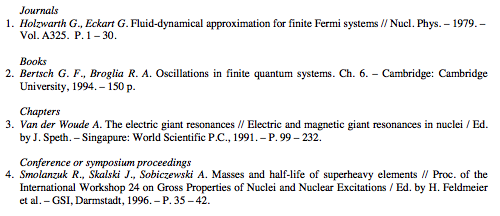
\includegraphics[width=0.500\linewidth]{example1a.png}

With Bibulous, we can easily provide templates that provide the formatting that the OP asks for::

\begin{Verbatim}[commandchars=\\\{\}]
TEMPLATES:
article = \PYGZbs{}textit\PYGZob{}\textless{}au\textgreater{}\PYGZcb{} \textless{}title\textgreater{} // \textless{}journal\textgreater{} -- \textless{}year\textgreater{}. -- Vol.\textasciitilde{}\textless{}volume\textgreater{}. P.\textasciitilde{}[\textless{}startpage\textgreater{} -- \textless{}endpage\textgreater{}\textbar{}\textless{}startpage\textgreater{}\textbar{}\textless{}eid\textgreater{}\textbar{}].
book = \PYGZbs{}textit\PYGZob{}\textless{}au\textgreater{}\PYGZcb{} \textless{}title\textgreater{}. [Ch.\textasciitilde{}\textless{}chapter\textgreater{}. ]-- \textless{}address\textgreater{}: \textless{}publisher\textgreater{}, \textless{}year\textgreater{}.[ -- \textless{}startpage\textgreater{}\textasciitilde{}p.]
inbook = \PYGZbs{}textit\PYGZob{}\textless{}au\textgreater{}\PYGZcb{} \textless{}title\textgreater{} // \textless{}booktitle\textgreater{}[ / Ed. by \textless{}ed.if\_singular(editorlist, nothing, etal\_message)\textgreater{}]. -- \textless{}address\textgreater{}: ...
         \textless{}publisher\textgreater{}, \textless{}year\textgreater{}.[ -- P.\textasciitilde{}\textless{}startpage\textgreater{} -- \textless{}endpage\textgreater{}\textbar{} -- P.\textasciitilde{}\textless{}startpage\textgreater{}\textbar{} -- P.\textasciitilde{}\textless{}eid\textgreater{}\textbar{}].
inproceedings = \PYGZbs{}textit\PYGZob{}\textless{}au\textgreater{}\PYGZcb{} \textless{}title\textgreater{} // \textless{}booktitle\textgreater{}[ / Ed. by \textless{}ed.if\_singular(editorlist, nothing, etal\_message)\textgreater{}]. -- ...
         \textless{}publisher\textgreater{}, \textless{}address\textgreater{}, \textless{}year\textgreater{}. -- P.\textasciitilde{}[\textless{}startpage\textgreater{} -- \textless{}endpage\textgreater{}\textbar{}\textless{}startpage\textgreater{}\textbar{}\textless{}eid\textgreater{}\textbar{}].

SPECIAL-TEMPLATES:
authorlist = \textless{}author.to\_namelist()\textgreater{}
editorlist = \textless{}editor.to\_namelist()\textgreater{}
authorname.n = [\textless{}authorlist.n.prefix\textgreater{} ]\textless{}authorlist.n.last\textgreater{}[ \textless{}authorlist.n.first.initial()\textgreater{}.][ \textless{}authorlist.n.middle.initial()\textgreater{}.][,  \textless{}authorlist.n.suffix\textgreater{}.]
au = \textless{}authorname.0\textgreater{}, ..., \textless{}authorname.9\textgreater{}
ed = [\textless{}editorlist.0.first.initial()\textgreater{}. ][ \textless{}editorlist.0.middle.initial()\textgreater{}. ][\textless{}editorlist.0.prefix\textgreater{} ]\textless{}editorlist.0.last\textgreater{}[,  \textless{}editorlist.0.suffix\textgreater{}.]

OPTIONS:
nothing = \PYGZob{}\PYGZcb{}
\end{Verbatim}

so that if we use this template together with the following database file:

\begin{Verbatim}[commandchars=\\\{\}]
@article\PYGZob{}Holzwarth,
  author = \PYGZob{}G. Holzwarth and G. Eckart\PYGZcb{},
  title = \PYGZob{}Fluid-dynamical approximation for finite Fermi systems\PYGZcb{},
  journal = \PYGZob{}Nucl. Phys.\PYGZcb{},
  year = 1979,
  volume = \PYGZob{}A325\PYGZcb{},
  pages = \PYGZob{}1-30\PYGZcb{}
\PYGZcb{}
@book\PYGZob{}Bertsch,
  author = \PYGZob{}G. F. Bertsch and R. A. Broglia\PYGZcb{},
  title = \PYGZob{}Oscillations in finite quantum systems\PYGZcb{},
  chapter = 6,
  address = \PYGZob{}Cambridge\PYGZcb{},
  publisher = \PYGZob{}Cambridge University\PYGZcb{},
  year = 1994,
  pages = 150
\PYGZcb{}
@inbook\PYGZob{}Woude,
  author = \PYGZob{}A. Van der Woude\PYGZcb{},
  title = \PYGZob{}The electric giant resonances\PYGZcb{},
  booktitle = \PYGZob{}Electric and magnetic giant resonances in nuclei\PYGZcb{},
  editor = \PYGZob{}J. Speth\PYGZcb{},
  address = \PYGZob{}Singapore\PYGZcb{},
  publisher = \PYGZob{}World Scientific P.C.\PYGZcb{},
  year = 1991,
  pages = \PYGZob{}99-232\PYGZcb{}
\PYGZcb{}
@inproceedings\PYGZob{}Smolanzuk,
  author = \PYGZob{}R. Smolanzuk and J. Skalski and A. Sobiczewski\PYGZcb{},
  title = \PYGZob{}Masses and half-life of superheavy elements\PYGZcb{},
  booktitle = \PYGZob{}Proc.\PYGZbs{} of the International Workshop 24 on Gross Properties of Nuclei and Nuclear Excitations\PYGZcb{},
  editor = \PYGZob{}H. Feldmeier and others\PYGZcb{},
  address = \PYGZob{}Darmstadt\PYGZcb{},
  publisher = \PYGZob{}GSI\PYGZcb{},
  year = 1996,
  pages = \PYGZob{}35-42\PYGZcb{}
\PYGZcb{}
\end{Verbatim}

then we get the formatted result shown below

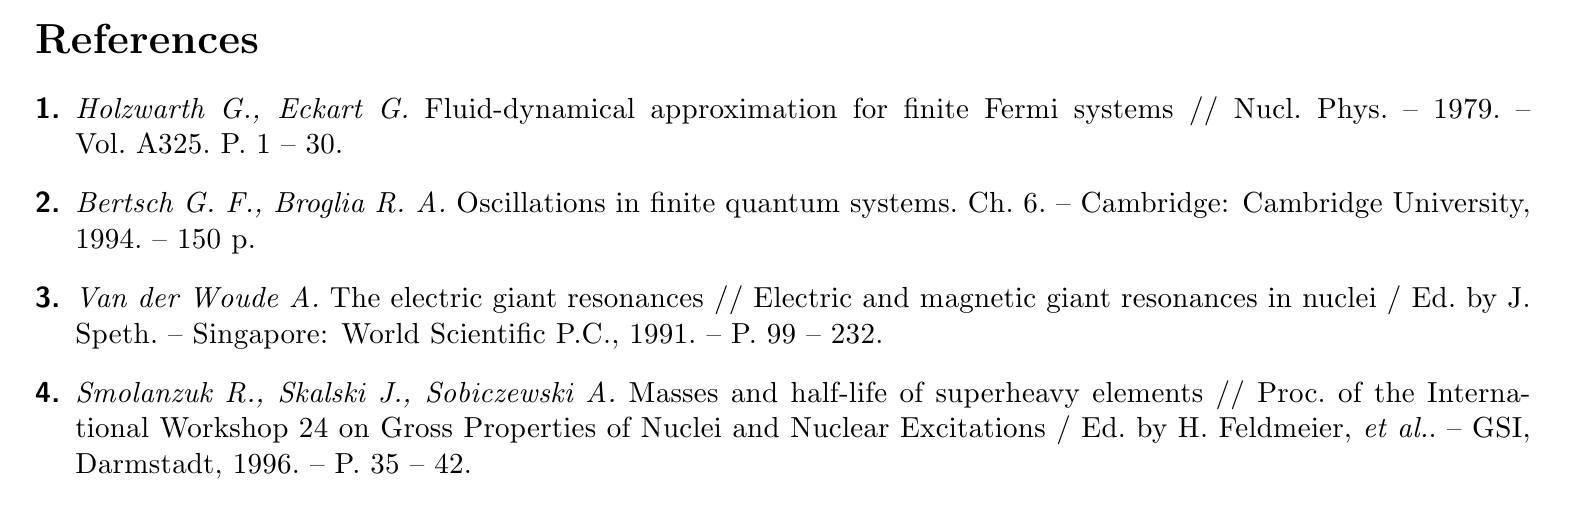
\includegraphics[width=0.600\linewidth]{example1b.png}


\bigskip\hrule{}\bigskip



\section{Example 2}
\label{examples:example-2}
The next example is taken from the bibliography style found in: Dimitri Mihalas and James Binney, \_Galactic Astronomy: Structure and {\color{red}\bfseries{}Kinematics\_}, 2nd ed. (W. H. Freeman, New York, 1981). A snapshot from the the book's bibliography looks like

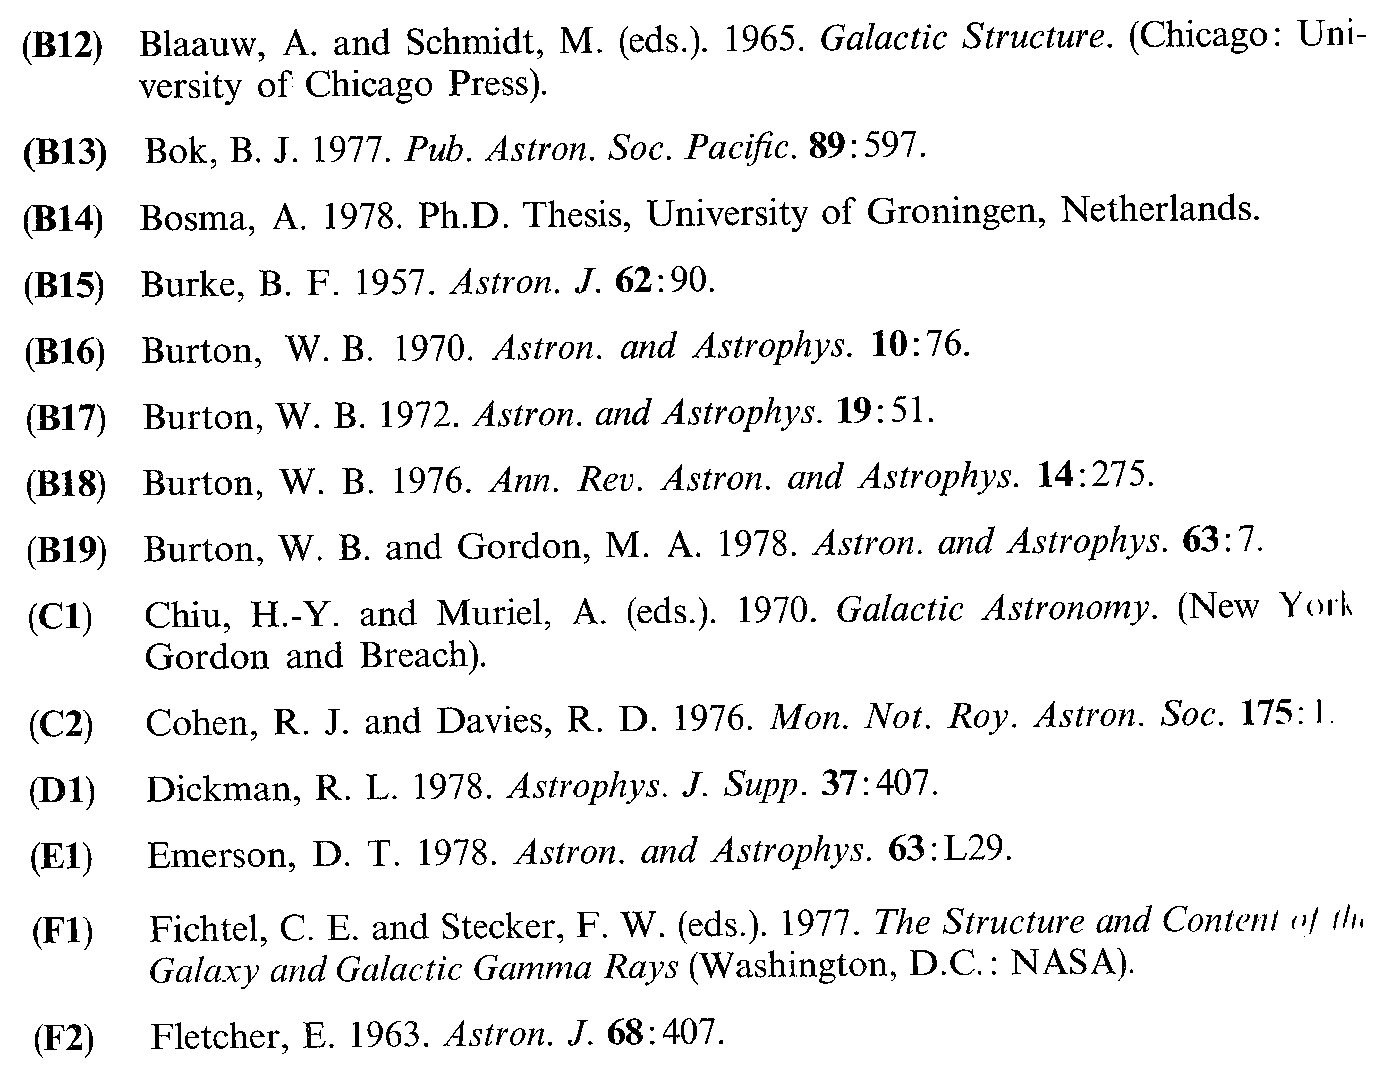
\includegraphics[width=0.500\linewidth]{example2a.png}

To produce this style, we can define the following templates::

\begin{Verbatim}[commandchars=\\\{\}]
TEMPLATES:
article = \textless{}au\textgreater{} \textless{}year\textgreater{}. \PYGZbs{}textit\PYGZob{}\textless{}journal\textgreater{}\PYGZcb{} \PYGZbs{}textbf\PYGZob{}\textless{}volume\textgreater{}\PYGZcb{}:\textless{}pages\textgreater{}.
book = [\textless{}au\textgreater{}\textbar{}\textless{}ed.if\_singular(editorlist, eds\_msg1, eds\_msg2)\textgreater{}\textbar{}]. \textless{}year\textgreater{}. \PYGZbs{}textit\PYGZob{}\textless{}title\textgreater{}\PYGZcb{}. (\textless{}address\textgreater{}: \textless{}publisher\textgreater{}).
proceedings = book
phdthesis = \textless{}au\textgreater{} \textless{}year\textgreater{}. Ph.D. Thesis, \textless{}university\textgreater{}.

SPECIAL-TEMPLATES:
authorlist = \textless{}author.to\_namelist()\textgreater{}
editorlist = \textless{}editor.to\_namelist()\textgreater{}
authorname.n = [\textless{}authorlist.n.prefix\textgreater{} ]\textless{}authorlist.n.last\textgreater{}[, \textless{}authorlist.n.first.initial()\textgreater{}.][ \textless{}authorlist.n.middle.initial()\textgreater{}.][,  \textless{}authorlist.n.suffix\textgreater{}.]
au = \textless{}authorname.0\textgreater{}, ...,\PYGZob{} and \PYGZcb{}\textless{}authorname.9\textgreater{}
editorname.n = [\textless{}editorlist.n.prefix\textgreater{} ]\textless{}editorlist.n.last\textgreater{}[, \textless{}editorlist.n.first.initial()\textgreater{}.][ \textless{}editorlist.n.middle.initial()\textgreater{}.][,  \textless{}editorlist.n.suffix\textgreater{}.]
ed = \textless{}editorname.0\textgreater{}, ...,\PYGZob{} and \PYGZcb{}\textless{}editorname.5\textgreater{}
authorlabel = [\textless{}authorlist.0.prefix\textgreater{}\textbar{}\textless{}authorlist.0.last\textgreater{}]
editorlabel = [\textless{}editorlist.0.prefix\textgreater{}\textbar{}\textless{}editorlist.0.last\textgreater{}]
sortkey = [\textless{}authorlabel\textgreater{}\textless{}year\textgreater{}\textbar{}\textless{}editorlabel\textgreater{}\textless{}year\textgreater{}]
citelabel = (\textless{}sortkey.initial()\textgreater{})

OPTIONS:
eds\_msg1 = \PYGZob{} \PYGZcb{}(ed.)
eds\_msg2 = \PYGZob{} \PYGZcb{}(eds.)
use\_citeextract = False
\end{Verbatim}

so that with the following database file:

\begin{Verbatim}[commandchars=\\\{\}]
@book\PYGZob{}Blaauw1965,
  editor = \PYGZob{}A. Blaauw and M. Schmidt\PYGZcb{},
  title = \PYGZob{}Galactic Structure\PYGZcb{},
  address = \PYGZob{}Chicago\PYGZcb{},
  publisher = \PYGZob{}University of Chicago Press\PYGZcb{},
  year = 1965
\PYGZcb{}
@article\PYGZob{}Bok1977,
  author = \PYGZob{}B. J. Bok\PYGZcb{},
  journal = \PYGZob{}Publ. Astron. Soc. Pacific\PYGZcb{},
  year = 1977,
  volume = 89,
  pages = 597
\PYGZcb{}
@phdthesis\PYGZob{}Bosma1978,
  author = \PYGZob{}A. Bosma\PYGZcb{},
  university = \PYGZob{}University of Groningen, Netherlands\PYGZcb{},
  year = 1978
\PYGZcb{}
@article\PYGZob{}Burke1957,
  author = \PYGZob{}B. F. Burke\PYGZcb{},
  journal = \PYGZob{}Astron. J.\PYGZcb{},
  year = 1957,
  volume = 62,
  pages = 90
\PYGZcb{}
@article\PYGZob{}Burton1970,
  author = \PYGZob{}W. B. Burton\PYGZcb{},
  journal = \PYGZob{}Astron. and Astrophys.\PYGZcb{},
  year = 1970,
  volume = 10,
  pages = 76
\PYGZcb{}
@article\PYGZob{}Burton1972,
  author = \PYGZob{}W. B. Burton\PYGZcb{},
  journal = \PYGZob{}Astron. and Astrophys.\PYGZcb{},
  year = 1972,
  volume = 19,
  pages = 51
\PYGZcb{}
@article\PYGZob{}Burton1976,
  author = \PYGZob{}W. B. Burton\PYGZcb{},
  journal = \PYGZob{}Ann. Rev. Astron. and Astrophys.\PYGZcb{},
  year = 1976,
  volume = 14,
  pages = 275
\PYGZcb{}
@article\PYGZob{}Burton1978,
  author = \PYGZob{}W. B. Burton and M. A. Gordon\PYGZcb{},
  journal = \PYGZob{}Astron. and Astrophys.\PYGZcb{},
  year = 1978,
  volume = 63,
  pages = 7
\PYGZcb{}
@book\PYGZob{}Chiu1970,
  editor = \PYGZob{}H.-Y. Chiu and A. Muriel\PYGZcb{},
  title = \PYGZob{}Galactic Astronomy\PYGZcb{},
  year = 1970,
  address = \PYGZob{}New York\PYGZcb{},
  publisher = \PYGZob{}Gordon and Breach\PYGZcb{}
\PYGZcb{}
@article\PYGZob{}Cohen1976,
  author = \PYGZob{}R. J. Cohen and R. D. Davies\PYGZcb{},
  journal = \PYGZob{}Mon. Not. Roy. Astron. Soc.\PYGZcb{},
  year = 1976,
  volume = 175,
  pages = 1
\PYGZcb{}
@article\PYGZob{}Dickman1978,
  author = \PYGZob{}R. L. Dickman\PYGZcb{},
  journal = \PYGZob{}Astrophys. J. Supp.\PYGZcb{},
  year = 1978,
  volume = 37,
  pages = 407
\PYGZcb{}
@article\PYGZob{}Emerson1978,
  author = \PYGZob{}D. T. Emerson\PYGZcb{},
  journal = \PYGZob{}Astron. and Astrophys.\PYGZcb{},
  year = 1978,
  volume = 63,
  pages = \PYGZob{}L29\PYGZcb{},
\PYGZcb{}
@inproceedings\PYGZob{}Fichtel1977,
  editor = \PYGZob{}C. E. Fichtel and F. W. Stecker\PYGZcb{},
  booktitle = \PYGZob{}The Structure and Content of the Galaxy and Galactic Gamma Rays\PYGZcb{},
  address = \PYGZob{}Washington, D.C.\PYGZcb{},
  publisher = \PYGZob{}NASA\PYGZcb{},
  year = 1977
\PYGZcb{}
\end{Verbatim}

we get the following formatted result


\chapter{Bibulous Overview}
\label{index:bibulous-overview}
Bibulous is a drop-in replacement for BibTeX that makes use of style templates instead of BibTeX's BST language. The code is written in Python and, like BibTeX itself, is open source.

Bibulous developed out of frustration with the complexity of creating bibliography styles using BibTeX's obscure language, and also from the realization that because bibliographies are highly structured, one should be able to specify them simply and flexibly using a template approach. There should be no need to learn a new language just to build a bibliography style, and specifying a style should taken only a matter of minutes.

Bibulous incorporates this template approach, and at the same time implements many of the modern enhancements to BibTeX, such as the ability to work with languages other than English, better support for allowing non-standard bibliography entry types, increased options for author name formatting, and more. And one can use the same basic structures and LaTeX commands to generating each of: a bibliography, a glossary, an annotated bibliography, a list of acronyms and symbols, and more, by specifying a different style template for each case.

Bibulous' “style template” files allow a user to visualize the entire bibliography format structure in a concise way within a single page of text. Moreover, the template is structured with its own Python-like mini-language, intended to allow uses to create flexible formatting instructions quickly and easily. The example below illustrates the simplicity of the format.


\section{Installation}
\label{index:installation}
Installing using pip::

\begin{Verbatim}[commandchars=\\\{\}]
pip install bibulous
\end{Verbatim}

Instructions for installing Bibulous, and for seamlessly integrating it into your normal LaTeX workflow, are given in the \code{INSTALL.rst} file. Users can also consult the user guide (\code{user\_guide.rst}) for further information and tutorials. A \code{FAQ} page is also available.


\section{Example}
\label{index:example}
For a very simple bibliography, consisting of only journal articles and books, a complete style template file may consist of just two lines::

\begin{Verbatim}[commandchars=\\\{\}]
article = \textless{}au\textgreater{}, \PYGZbs{}enquote\PYGZob{}\textless{}title\textgreater{},\PYGZcb{} \PYGZbs{}textit\PYGZob{}\textless{}journal\textgreater{}\PYGZcb{} \PYGZbs{}textbf\PYGZob{}\textless{}volume\textgreater{}\PYGZcb{}: ...
             [\textless{}startpage\textgreater{}--\textless{}endpage\textgreater{}\textbar{}\textless{}startpage\textgreater{}\textbar{}\textless{}eid\textgreater{}\textbar{}] (\textless{}year\textgreater{}).[ \textless{}note\textgreater{}]
book = [\textless{}au\textgreater{}\textbar{}\textless{}ed\textgreater{}\textbar{}], \PYGZbs{}textit\PYGZob{}\textless{}title\textgreater{}\PYGZcb{} (\textless{}publisher\textgreater{}, \textless{}year\textgreater{})...
             [, pp.\textasciitilde{}\textless{}startpage\textgreater{}--\textless{}endpage\textgreater{}].[ \textless{}note\textgreater{}]
\end{Verbatim}

The \code{\textless{}variable\textgreater{}} notation indicates that the corresponding bibliography entry's field is to be inserted into the template there. The \code{{[}...\textbar{}...{]}} notation behaves similar to an if...elseif... statement, checking whether a given field is defined within the bibliography entry. If not defined, then it attempts to implement the instruction in the block following the next \code{\textbar{}} character.

We can read the above article template as indicating the following structure for LaTeX-formatting the cited entry in the bibliography (\code{.bib} file). For articles, we first insert the list of author names (formatted according to the default form), followed by a comma. If no \code{author} field was found in the bibliography entry, then insert \code{???} to indicate a missing required field. Next insert a quoted title, followed by an italicized journal name, and a boldface volume number (all of these are required fields). Next, if the \code{pages} field was found in the entry's database, then parse the start and end page numbers and insert them here. If the \code{pages} field indicates that there was only one page, then use that instead. Or if the \code{pages} field is not present, then check to see if the \code{eid} is defined, and use it instead. However, if none of these three possibilities are available, then insert the “missing field” indicator, \code{???}. Finally, put the year inside parentheses, and if the \code{note} field is defined in the entry, then add that to the end (following the period). If \code{note} is not defined, then just ignore it.

One can read the book template similarly, and find that it has different required and optional fields. The simplicity of the format allows one to customize databases to suit any use. For example, to use a bibliography entrytype \code{本} instead of \code{book}, then all that is necessary is to go into the template file and change \code{book} to \code{本}. If a user wishes to add a new field, such as \code{translator}, then if it has been added to the \code{.bib} database file, then all that is needed is to add some text to the template, such as \code{(\textless{}translator\textgreater{}, trans.)} to insert the field into every bibliography entry that has \code{translator} defined for that entrytype.


\section{Developers}
\label{index:developers}
Bibulous is a new project, and so it has until now been a solo effort. Anyone interested in helping out is welcome to join; just send an email to the developers mailing list and we will try to help you get involved and show you the ropes. And, this being the maintainer's first open source project, any suggestions by experienced developers are welcome.

Guidelines for developers are given in \code{developer\_guide.rst}, and includes an overview of the project's strategy and overall code structure. Note that a bug tracking system has not yet been set up for the project. HTML-based documentation is provided in \code{bibulous/doc/\_build/html/index.html}, and a corresponding PDF file in \code{bibulous/doc/\_build/latex/Bibulous.pdf}. The \code{setup.py} and \code{MANIFEST.in} files provided in the repository base directory are used to create a Python package using the \code{disutils} distribution utilities module.


\section{License}
\label{index:license}
Bibulous is released under the MIT/X11 license, meaning that it is free and open source, and that it can be used without restriction in other programs, commercial or not. The license is given in the file \code{LICENSE.txt}, the text of which is reproduced here:

Copyright (c) 2013 Bibulous developers

Permission is hereby granted, free of charge, to any person obtaining a copy of this software and
associated documentation files (the ``Software''), to deal in the Software without restriction,
including without limitation the rights to use, copy, modify, merge, publish, distribute,
sublicense, and/or sell copies of the Software, and to permit persons to whom the Software is
furnished to do so, subject to the following conditions:

The above copyright notice and this permission notice shall be included in all copies or
substantial portions of the Software.

THE SOFTWARE IS PROVIDED ``AS IS'', WITHOUT WARRANTY OF ANY KIND, EXPRESS OR IMPLIED, INCLUDING BUT
NOT LIMITED TO THE WARRANTIES OF MERCHANTABILITY, FITNESS FOR A PARTICULAR PURPOSE AND
NONINFRINGEMENT. IN NO EVENT SHALL THE AUTHORS OR COPYRIGHT HOLDERS BE LIABLE FOR ANY CLAIM,
DAMAGES OR OTHER LIABILITY, WHETHER IN AN ACTION OF CONTRACT, TORT OR OTHERWISE, ARISING FROM, OUT
OF OR IN CONNECTION WITH THE SOFTWARE OR THE USE OR OTHER DEALINGS IN THE SOFTWARE.


\section{Indices and tables}
\label{index:indices-and-tables}\begin{itemize}
\item {} 
\emph{genindex}

\item {} 
\emph{search}

\end{itemize}

\begin{longtable}{ll}
\hline
\endfirsthead

\multicolumn{2}{c}%
{{\bfseries \tablename\ \thetable{} -- continued from previous page}} \\
\hline
\endhead

\hline \multicolumn{2}{|r|}{{Continued on next page}} \\ \hline
\endfoot

\hline
\endlastfoot

\end{longtable}




\renewcommand{\indexname}{Index}
\printindex
\end{document}
